%
In this section, we validate our proposed NZ-WHO templates in two different ways. First, we make a set of NZ-WHO templates for a set of CAD models from various viewpoints. Then we run the bank of NZ-WHO templates as ensembles of weak detectors and show that the rendering image can be We want to see how robust the NZ-WHO to real images a

Second, we show that our method can complement the detection bounding boxes coming out of standard object detectors. This process will enrich object detection bounding boxes with 2D-3D matching which gives continuous viewpoint estimation, a CAD model (rendering, depth) and fine-grained category.  

\subsection{2D-3D Matching as an Object Detector} 

We created ensemble of NZ-WHO templates using 9 CAD models and measured the Average Precision (AP) of object detection task and Mean Precision in Pose Estimation (MPPE) \cite{Lopez-Sastre11}. MPPE is the average of viewpoint accuracy.  

% Instance-level 2D-3D matching (registration) is a difficult problem since we need a CAD model that looks similar to the object in the image. Especially, due to extreme intraclass variability of chair \cite{Aubry14} used a very large collection of CAD models to cover variety of chairs. Similarly, \cite{Lim14}

Our ensemble of NZ-WHO templates is generated from rendering images within few minutes but shows reasonable performance on object detection task. The baseline method are Aspect Layout Model (ALM) \cite{Xiang12} and VOC-DPM \cite{Pepik12}. Note that the baseline methods require complex 3D modeling and viewpoint annotated natural images.

The detection result is on Table \ref{tab:3dobject} and example output from our method is on Figure \ref{fig:3dobject}. 

\begin{table}[!htbp]
    \footnotesize
  \begin{center}
    \begin{tabular}{|c|c|c|c|}
    \hline
     AP/MPPE& Ours & ALM\cite{Xiang12} & VOC-DPM\cite{Pepik12} \\
    \hline\hline
    car & \textbf{99.8}/91.7 &  98.4/93.4 & \textbf{99.8}/\textbf{97.5} \\ 
    bicycle & 93.0/87.4 & 93.0/91.4 & \textbf{98.8}/\textbf{97.5} \\
    \hline
    \end{tabular}
  \end{center}
  \caption{Average Precision(AP) and Mean Precision in Pose Estimation (MPPE) on 3DObject dataset car category. Our method produces high quality 2D-3D matching yet performs on par with state-of-the art detectors.}
  \label{tab:3dobject}
\end{table}

\begin{figure}[h]
    \begin{center}
    \setlength\tabcolsep{0pt}
\begin{tabular}{cc}
  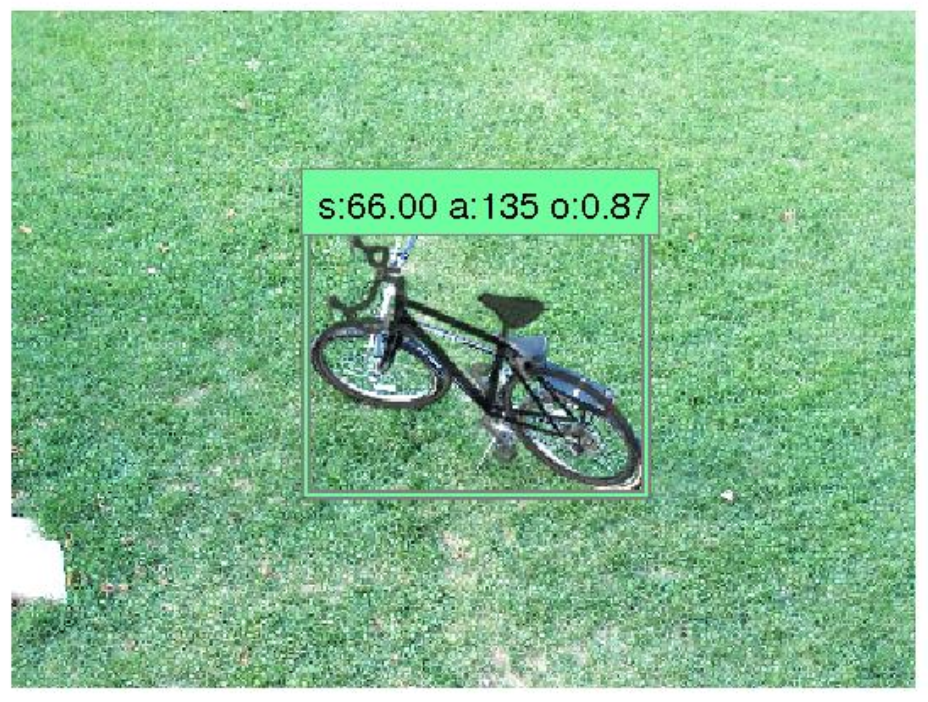
\includegraphics[width=0.45\linewidth]{car_3dobject/7.png} &   
  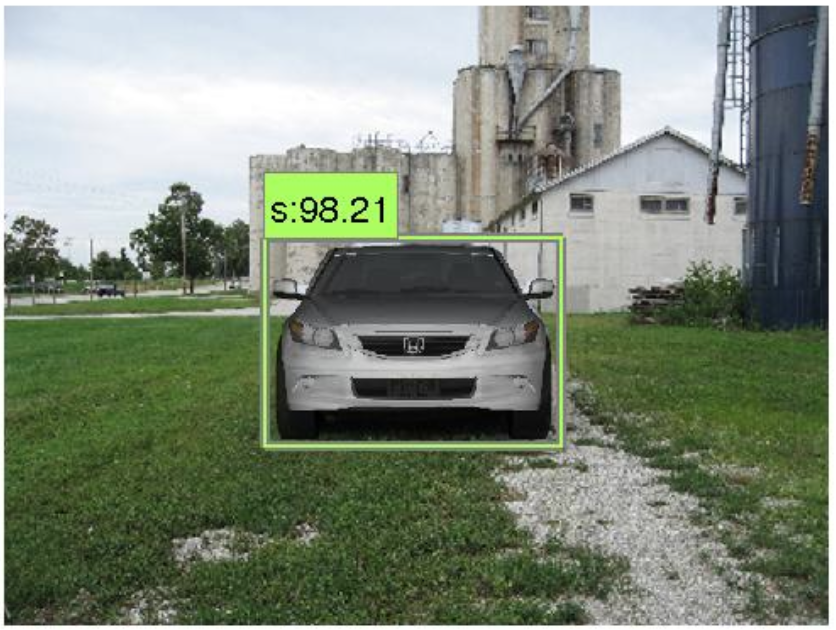
\includegraphics[width=0.45\linewidth]{car_3dobject/8.png}\\ [-15pt]
%   (a) & (b) \\[0pt]
  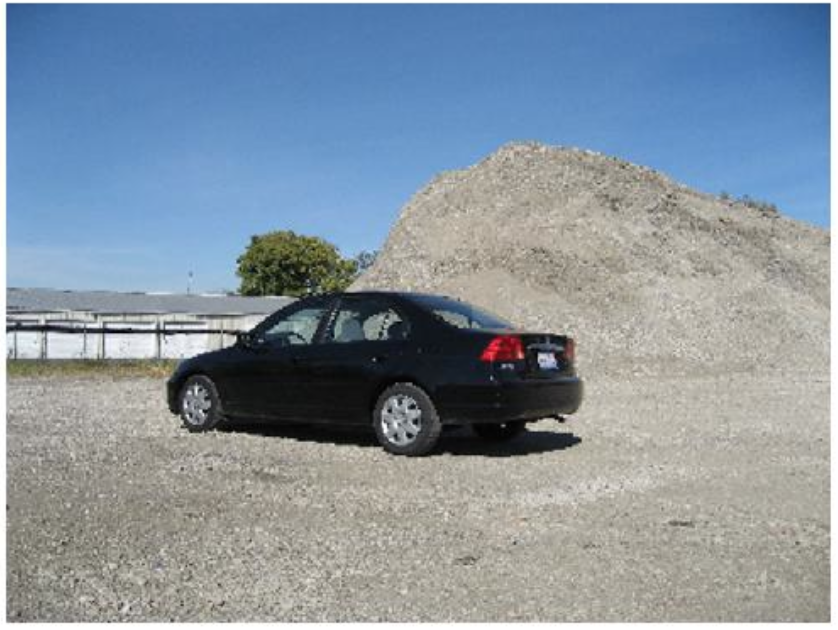
\includegraphics[width=0.45\linewidth]{car_3dobject/11.png} &   
  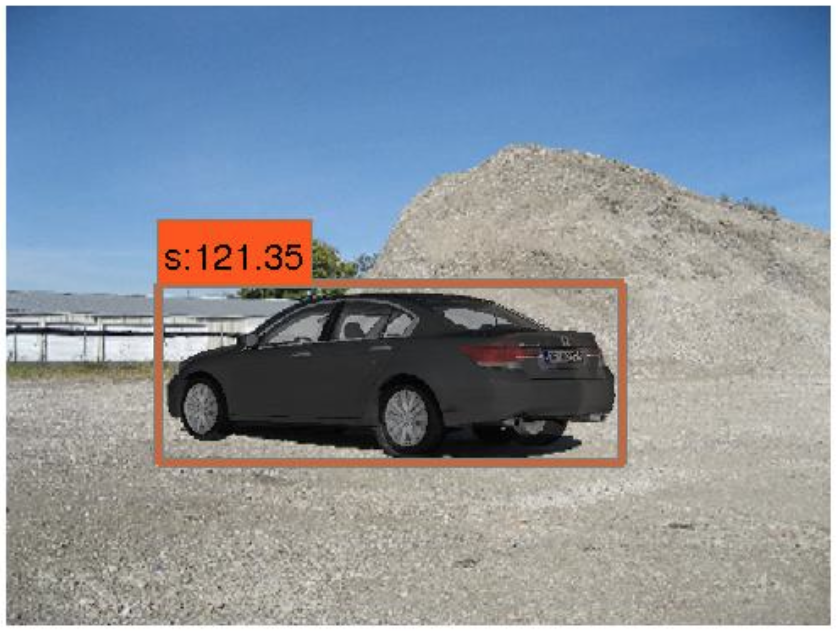
\includegraphics[width=0.45\linewidth]{car_3dobject/12.png}\\ [-5pt]
%  (c) & (d) \\[0pt]
\end{tabular}
\end{center}
\caption{Detection results on 3D-Object dataset \cite{Savarese07}. Original image (left) and detection result overlaid on top with a bounding box and corresponding confidence score(right)}
  \label{fig:3dobject}
\end{figure}


% Also, we evaluated our method on PASCAL 2007 dataset.
% 
% \begin{table}[!htbp]
%   \begin{center}
%   \begin{tabular}{|c|c|c|c|c|}
%     \hline
%      AP &    Ours &    ELDA \cite{Hariharan12} & ESVM \cite{Malisiewicz11} & VOCDPM \cite{Pepik12} \\
%     \hline\hline
%     car      & 27.          &  38.4  & 40.1    &65.7  \\ 
%     bicycle  & 43.74 & 41      &  40.7   & 61.3   \\
%     \hline
%     \end{tabular}
%   \end{center}
%   \caption{Average Precision(AP) on PASCAL 2007 dataset. Though we do not need any training images and made templates in few minues, it performs on par with state of the art detector yet it gives high quality 2D-3D matching.}
%   \label{tab:pascal07}
% \end{table}

\subsection{Fine-Tuning and Viewpoint Estimation}

High performance object detectors usually generalizes very well. It can handle various intraclass variability, viewpoint change and occlusion. However due to this high generalization, sometimes it is very difficult to get accurate pose, category or 2D-3D matching. Our method, specialized in giving such accurate information, can be applied on any generic object detectors to give high quality metadata.

To show such ability, we evaluated our method on PASCAL 3D dataset \cite{Xiang14}. The dataset augments PASCAL 2012 images with high quality viewpoint annotations thus is ideal to measure pose estimation. The dataset proposes new metric called Average Viewpoint Precision (AVP) where it measures the area under viewpoint precision and detection recall curve. The viewpoints is measured by azimuth similarity. If the distance between predicted azimuth and ground truth azimuth is below a certain threshold, the viewpoint is correct. Note that the baseline methods (V-DPM, VOC-DPM) reported on the PASCAL 3D dataset are variants of DPM where each component of DPM account for various azimuths. Thus V-DPM and VOC-DPM provide discrete azimuth only whereas our method provides 3D viewpoint (yaw, pitch, roll), CAD instance (model index, rendering, depth) and focal length.

We used detection bounding boxes and augment it using our method to give viewpoint estimation. We used detection bounding boxes from two different methods: VOC-DPM \cite{Pepik12} and R-CNN \cite{Girshick14}. VOC-DPM is a variation of DPM that can estimate viewpoint and is the state-of-the-art performance in viewpoint estimation \cite{Xiang14}. The result is on Table \ref{tab:pascal12} and precision recall curves for car using R-CNN + Ours are on Figure \ref{fig:car_cnn_ap}. 

We got significant improvement on viewpoint estimation by using our method on top of general purpose detectors. Note that our method estimates azimuth, elevation, in-plane rotation, focal length estimation, fine-grained categorization whereas V-DPM, VOC-DPM only estimate discrete viewpoints.

Example outputs are on Figure \ref{fig:pascal12cnn}.


\begin{figure*}[h]
\setlength\tabcolsep{1pt}
\centering
\begin{tabular}{|c|c|c|c|c|}
   \hline
  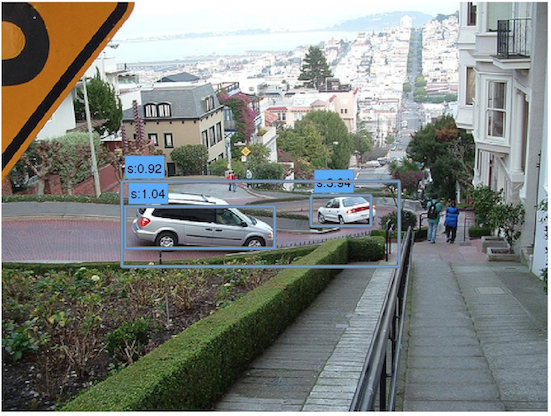
\includegraphics[width=0.24\textwidth]{car_cnn/1a.png} &   
  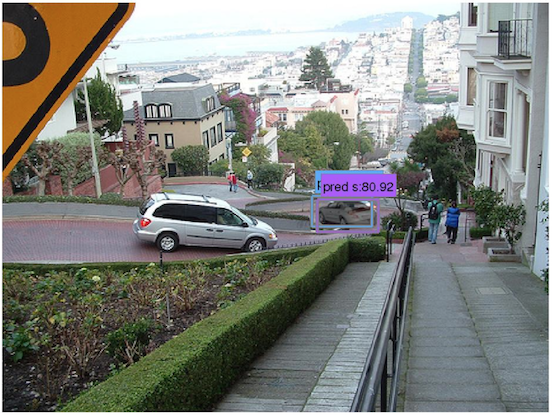
\includegraphics[width=0.24\textwidth]{car_cnn/1b.png} &   
  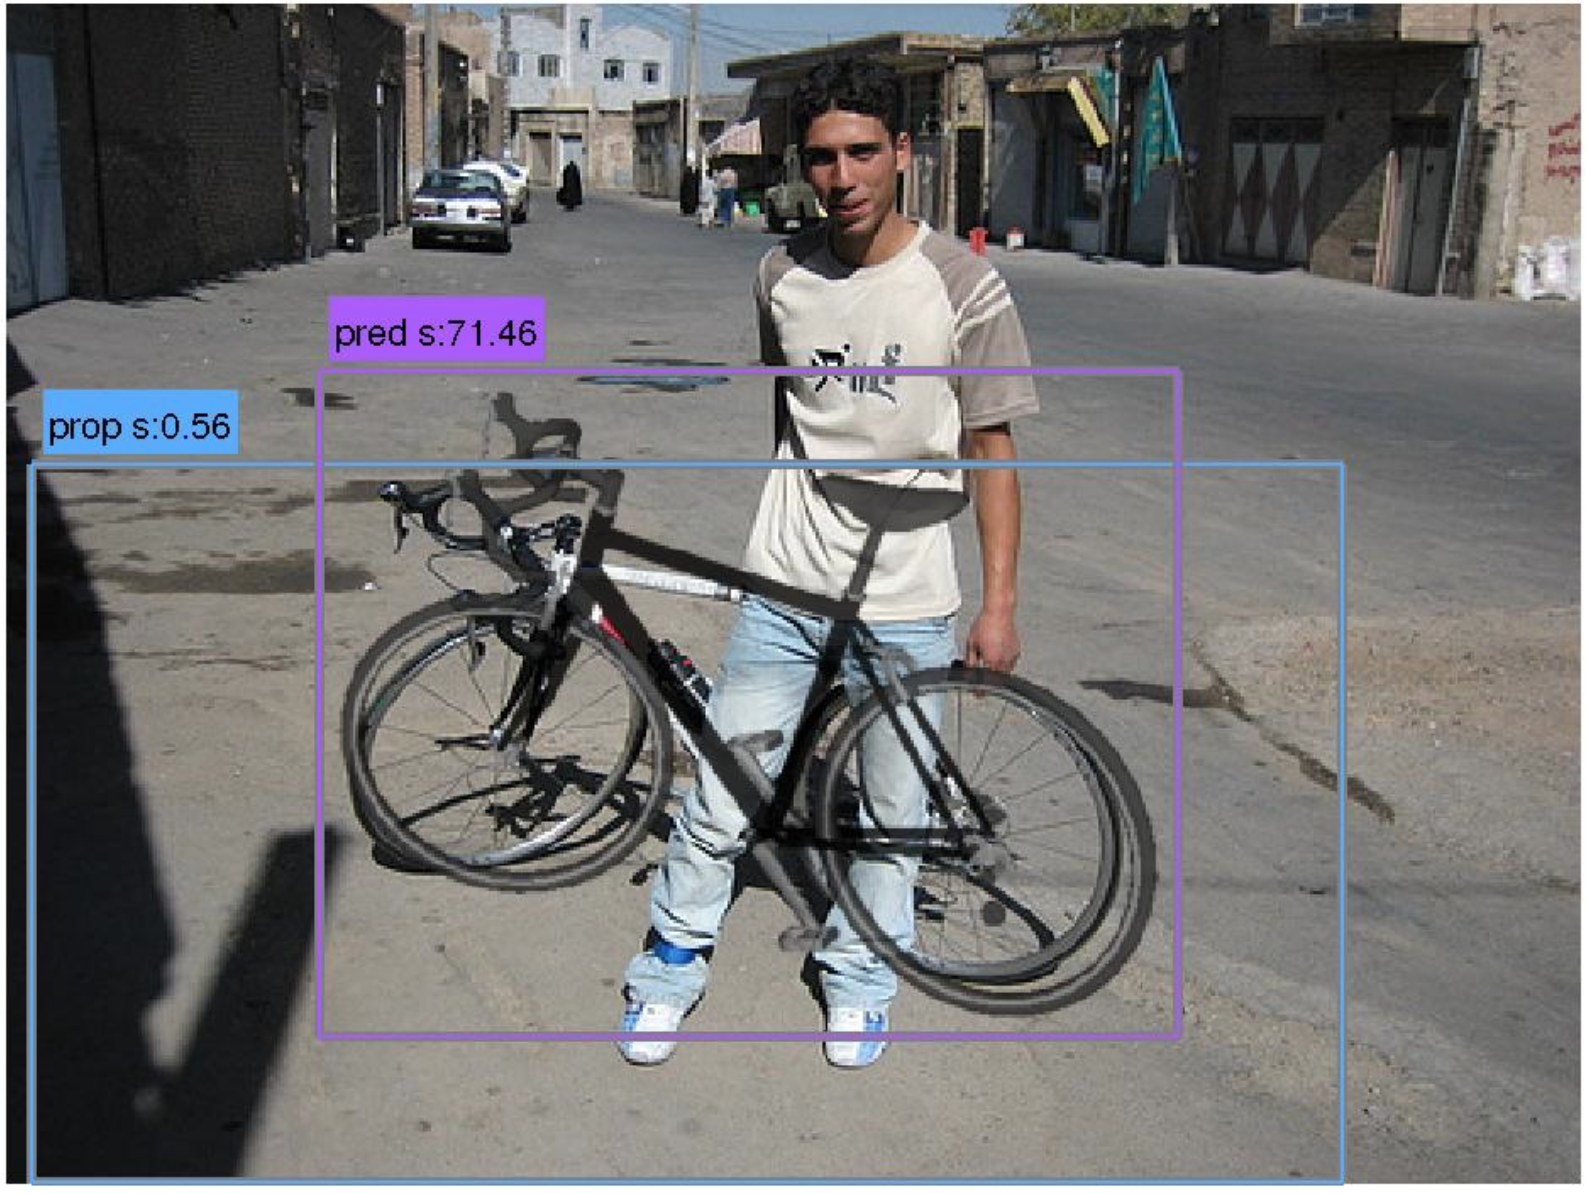
\includegraphics[width=0.24\textwidth]{car_cnn/1c.png} &   
  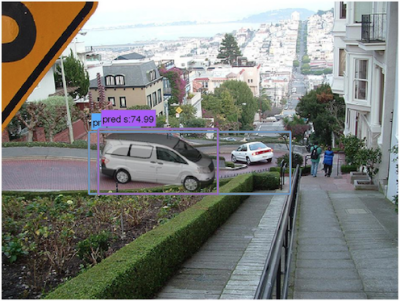
\includegraphics[width=0.24\textwidth]{car_cnn/1d.png}  \\  
   \hline
  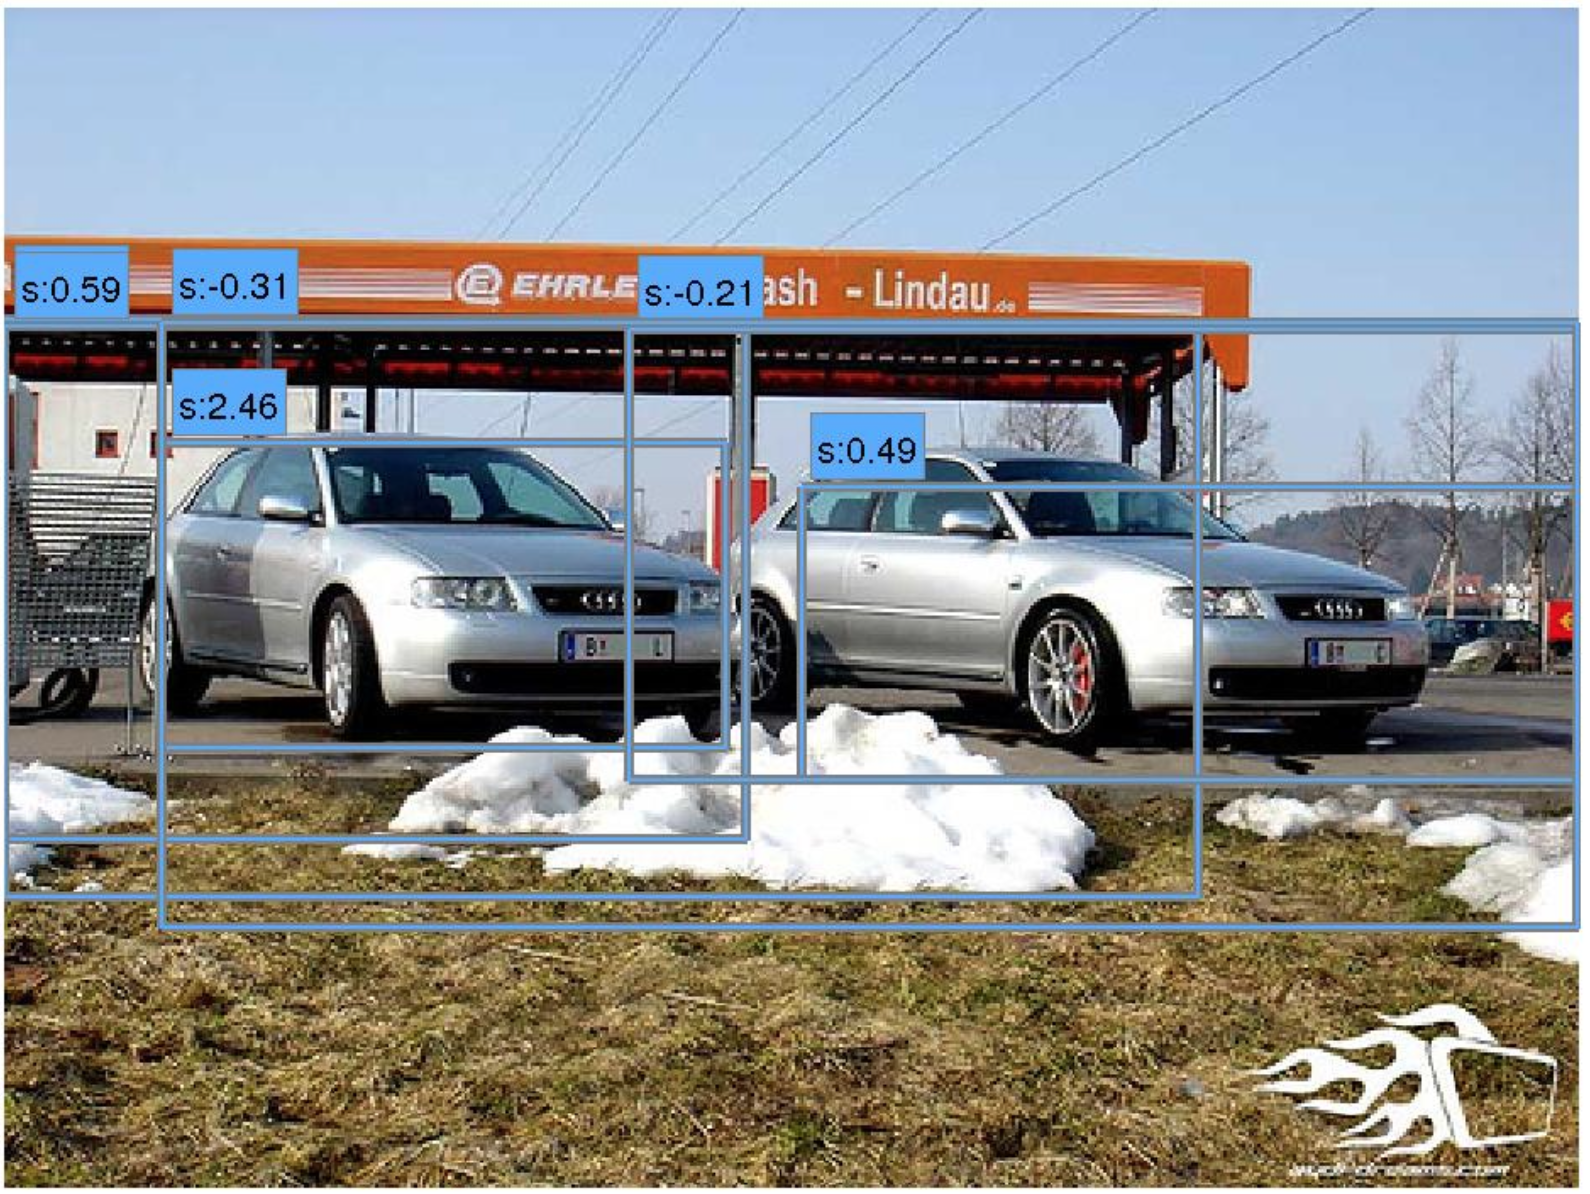
\includegraphics[width=0.24\textwidth]{car_cnn/2a.png} &   
  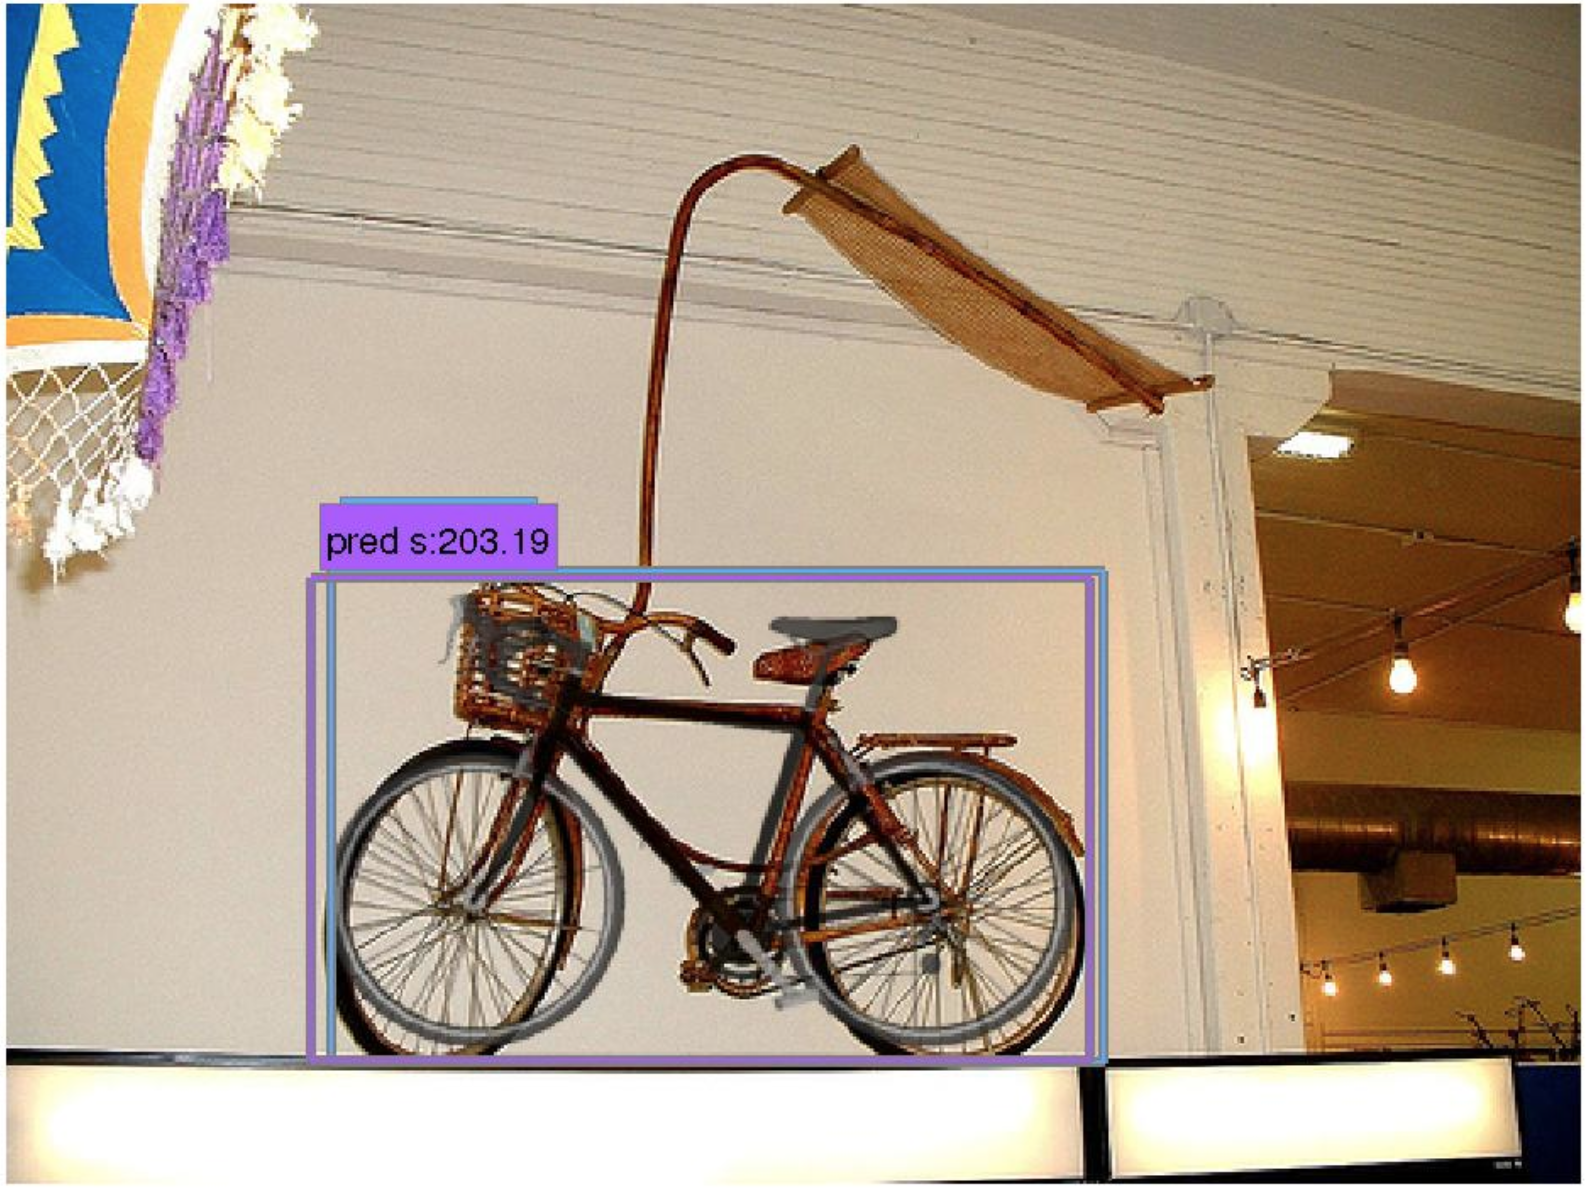
\includegraphics[width=0.24\textwidth]{car_cnn/2b.png} &   
  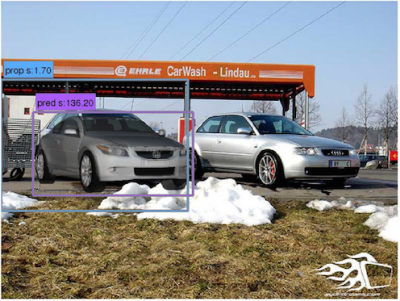
\includegraphics[width=0.24\textwidth]{car_cnn/2c.png} &   
  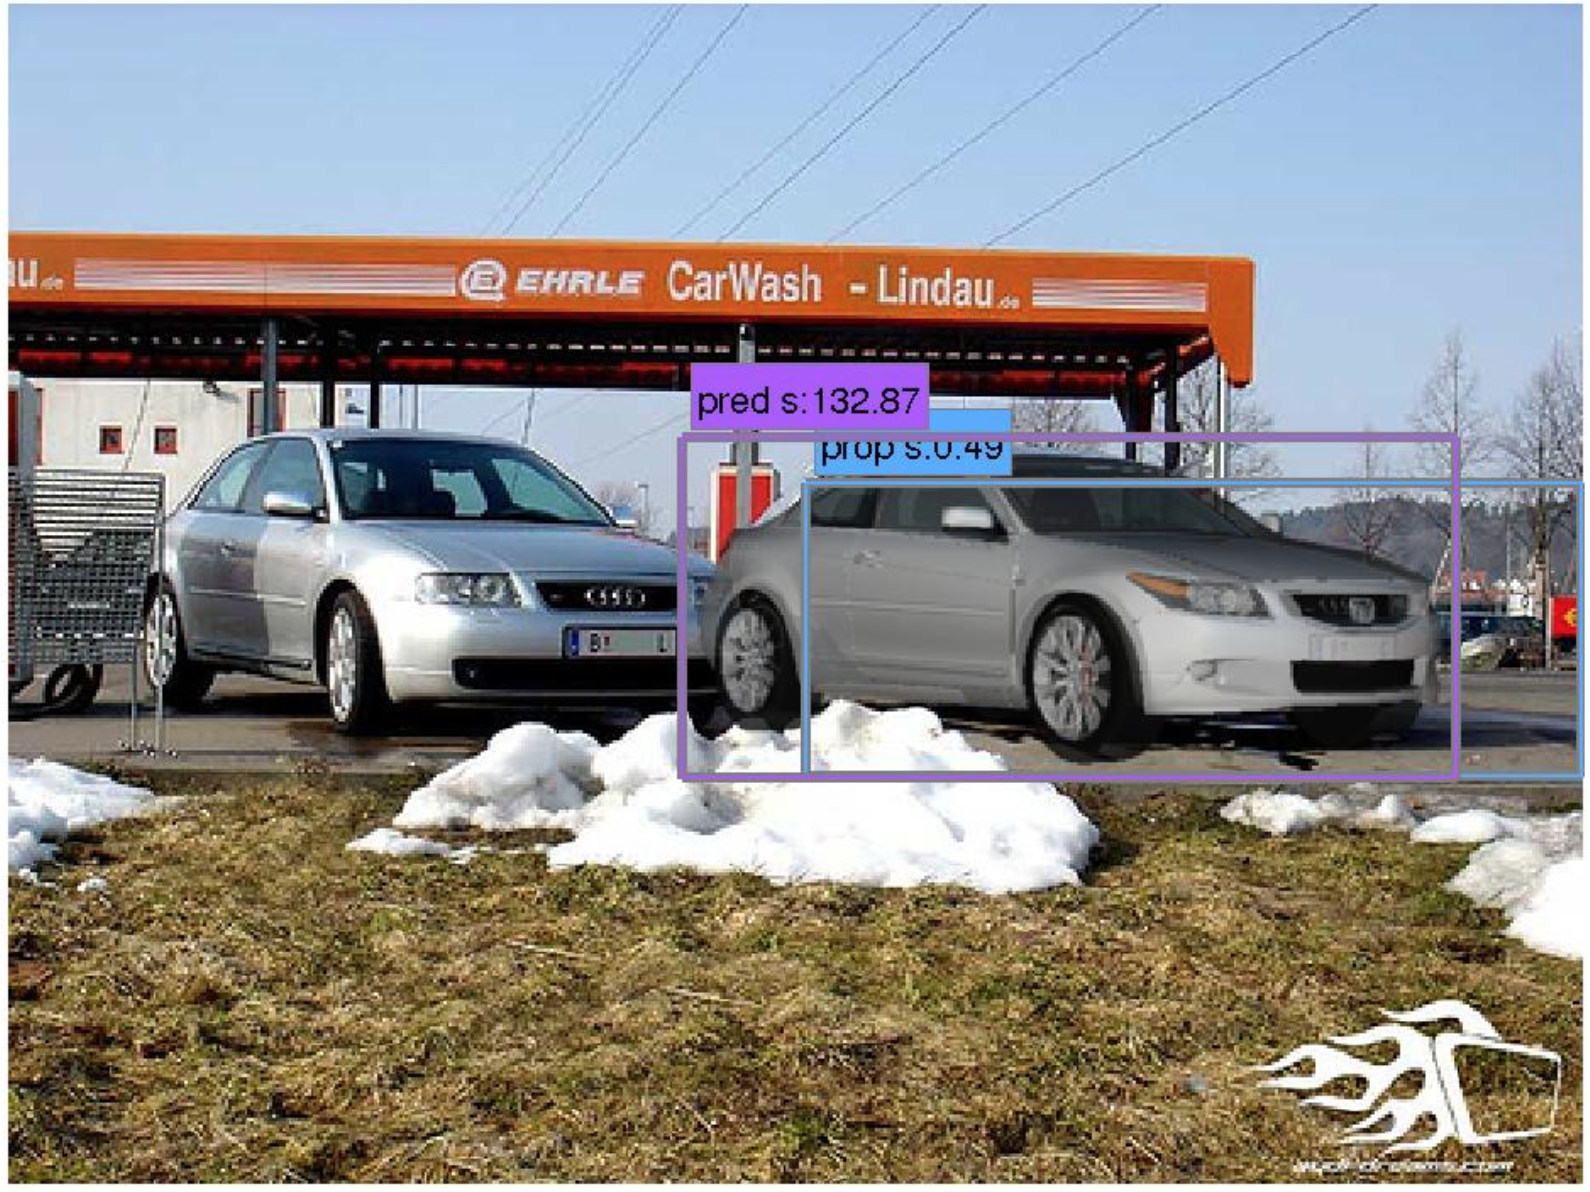
\includegraphics[width=0.24\textwidth]{car_cnn/2e.png}  \\  
   \hline
  \includegraphics[width=0.24\textwidth]{car_cnn/4a.png} &   
  \includegraphics[width=0.24\textwidth]{car_cnn/4b.png} &   
  \includegraphics[width=0.24\textwidth]{car_cnn/4c.png} &   
  \includegraphics[width=0.24\textwidth]{car_cnn/4d.png}  \\  
%    \hline
%   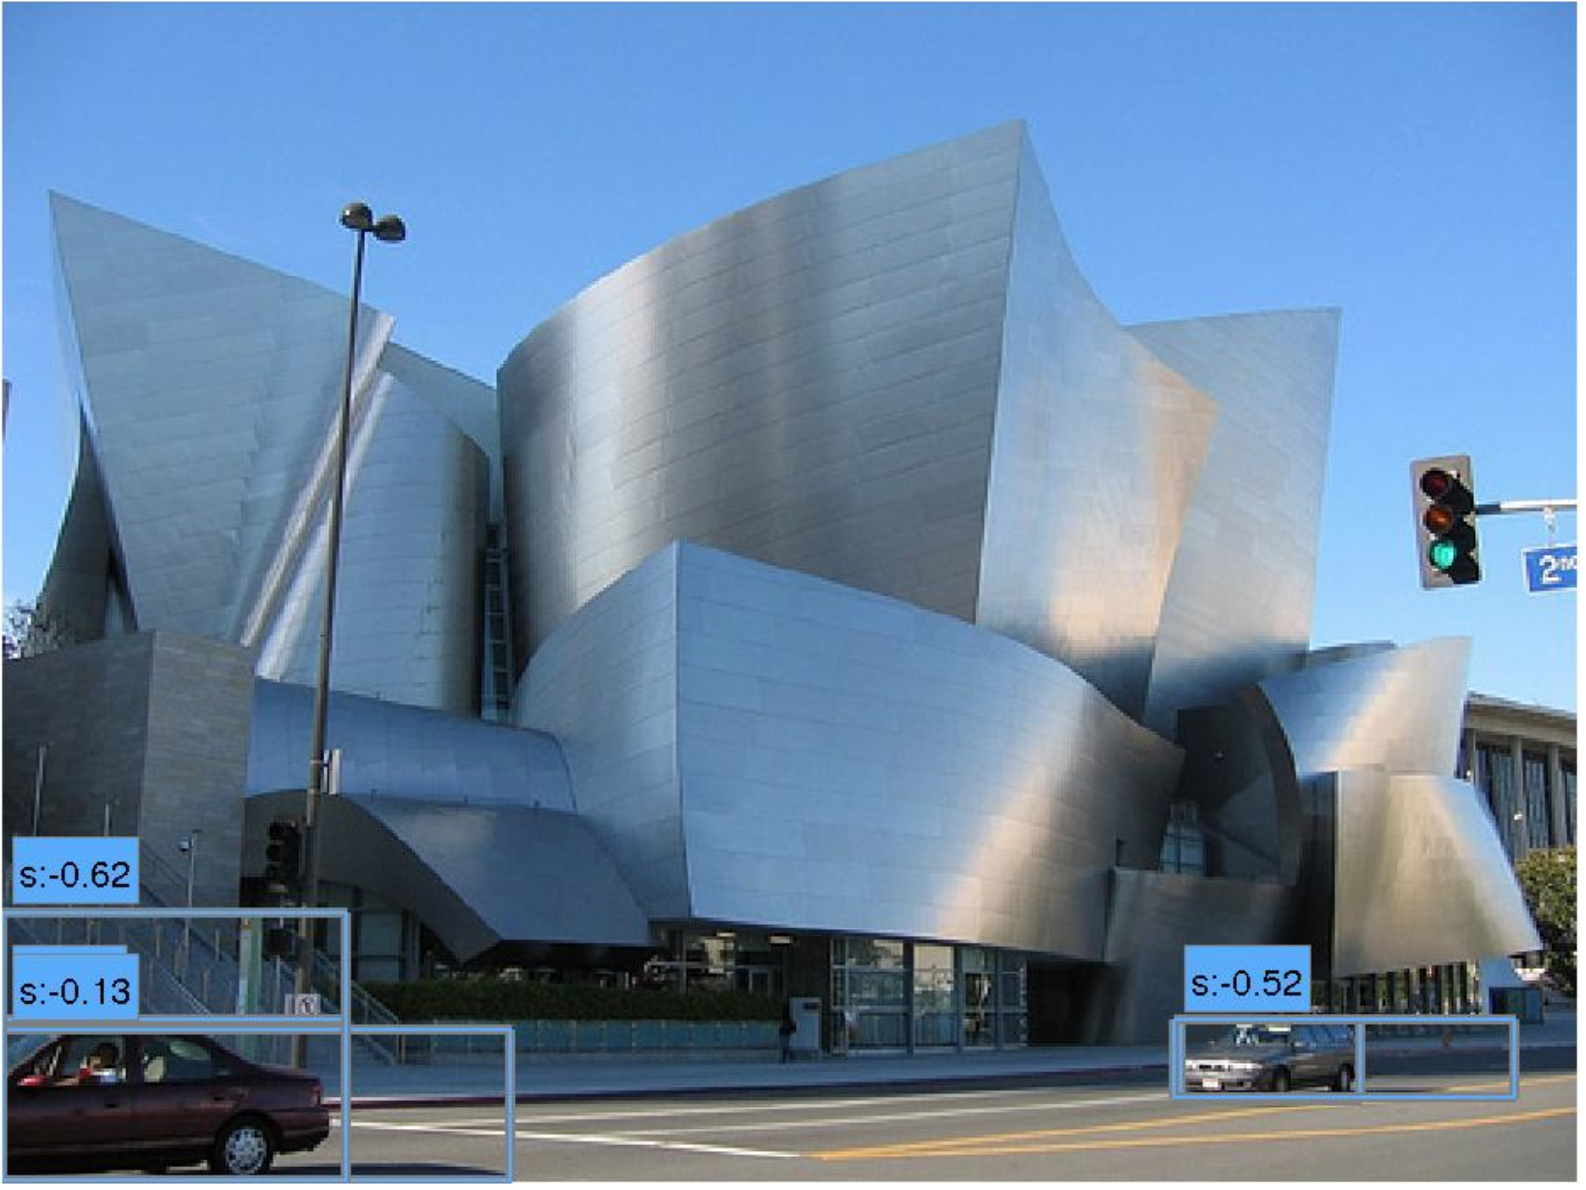
\includegraphics[width=0.24\textwidth]{car_cnn/10a.png} &   
%   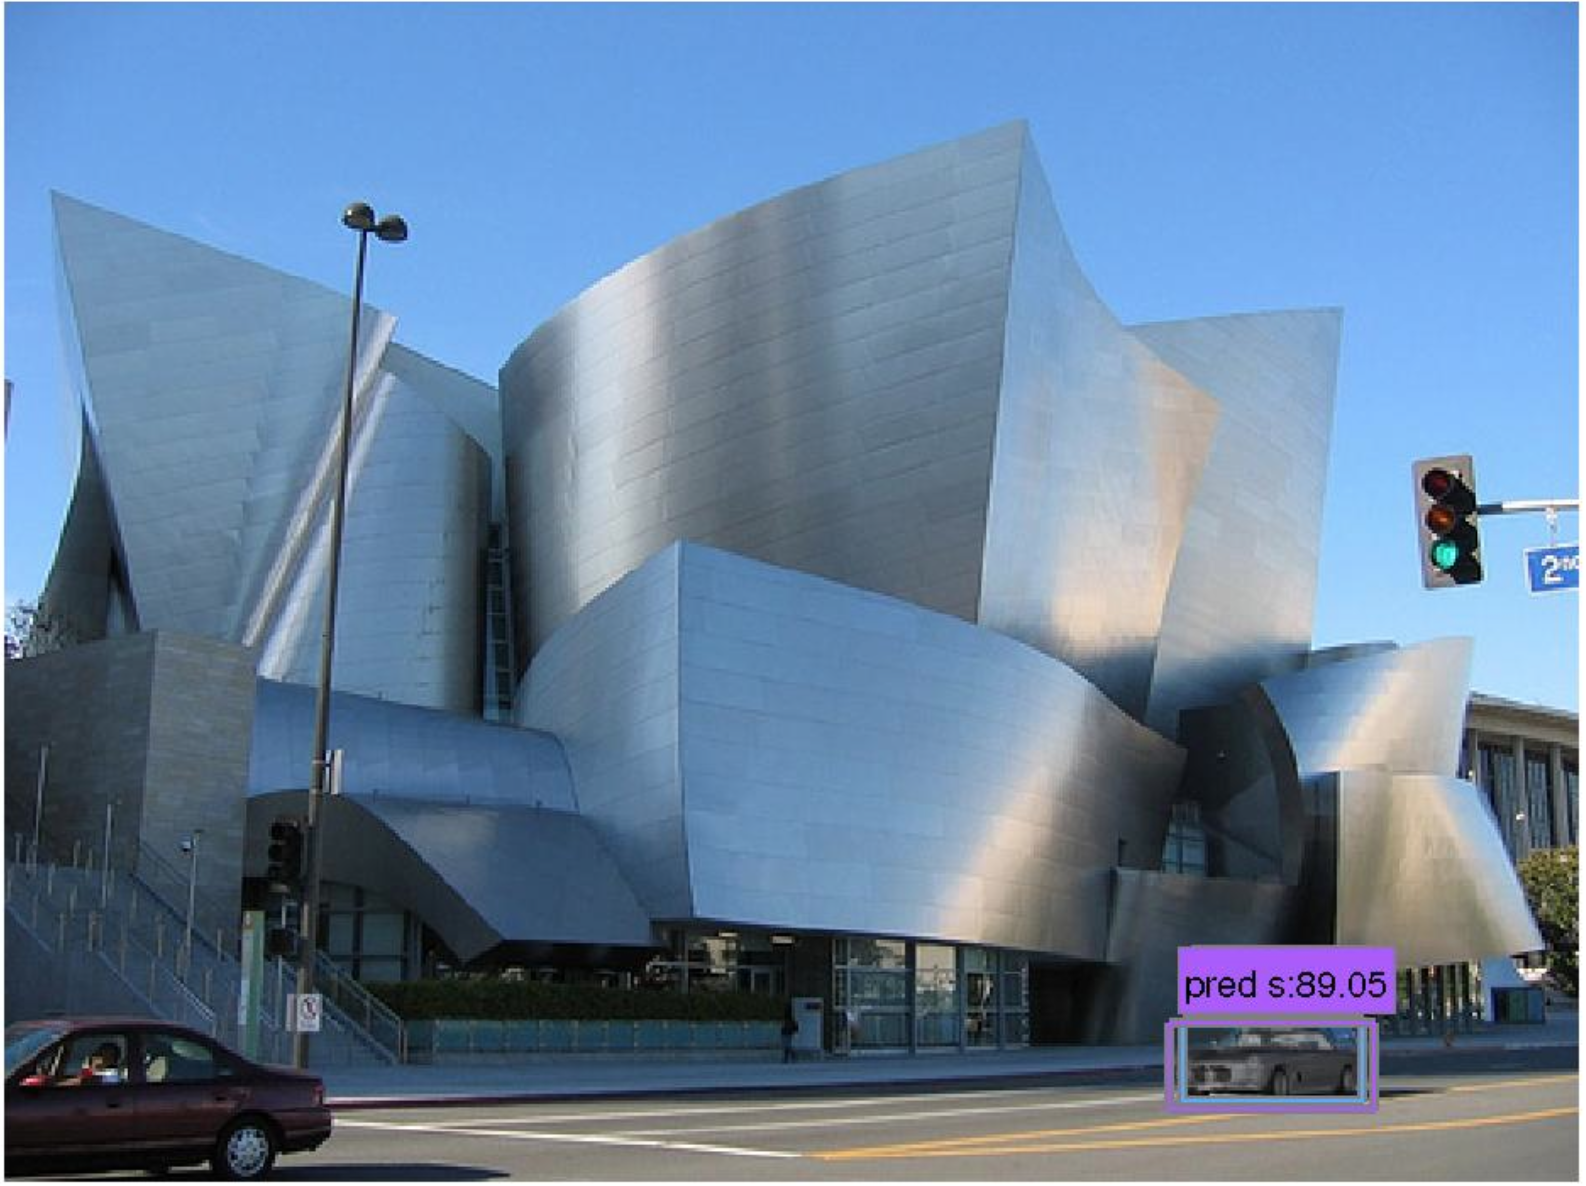
\includegraphics[width=0.24\textwidth]{car_cnn/10b.png} &   
%   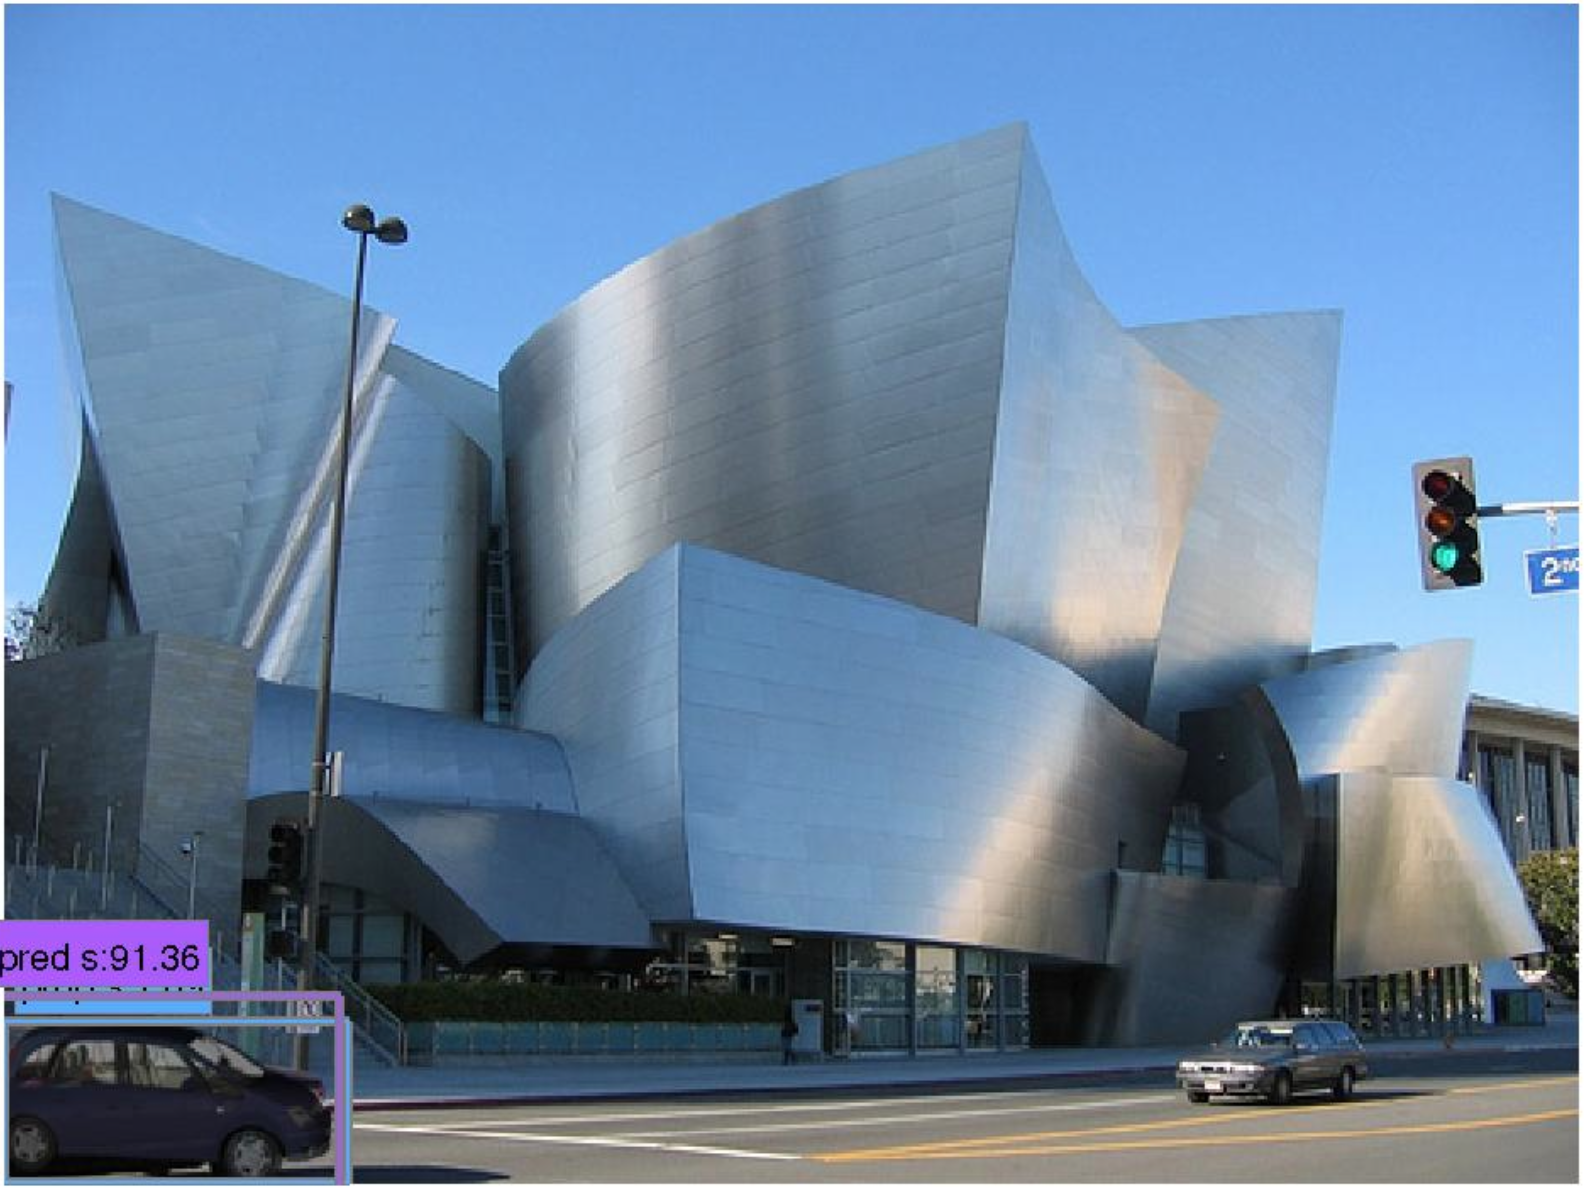
\includegraphics[width=0.24\textwidth]{car_cnn/10c.png} &   
%   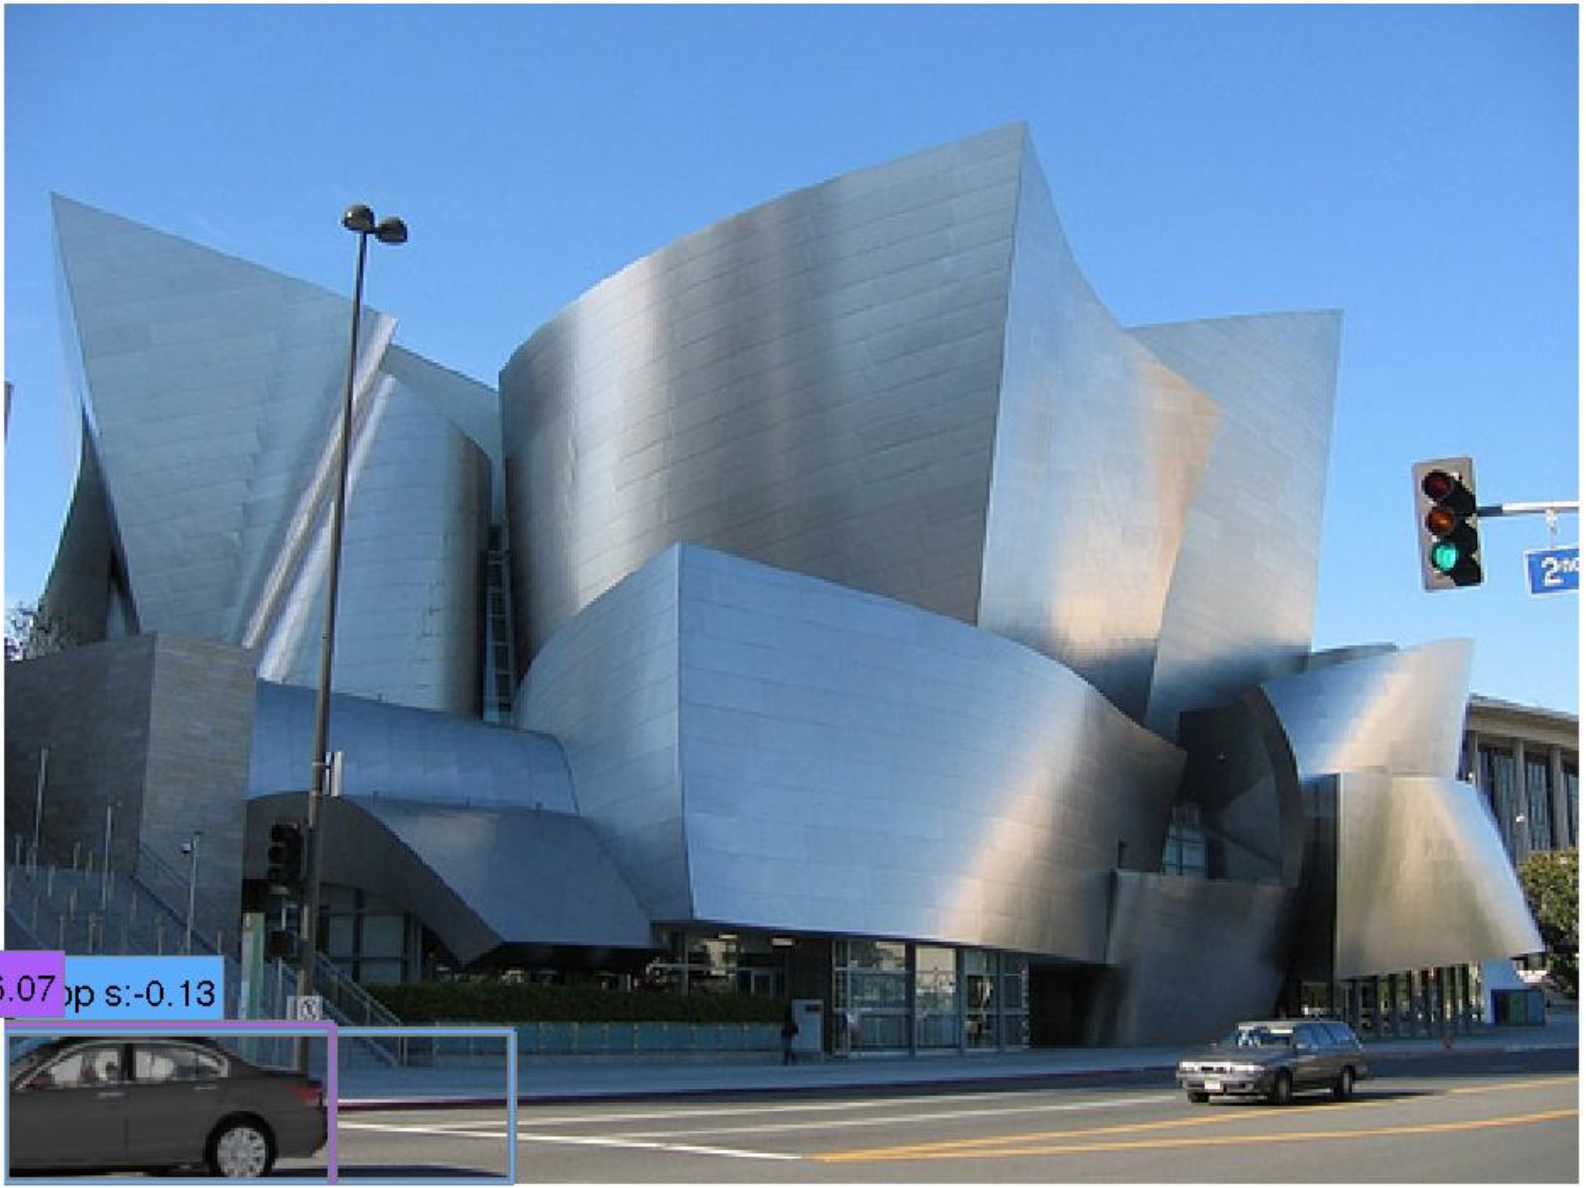
\includegraphics[width=0.24\textwidth]{car_cnn/10d.png}  \\  
%   \hline 
%   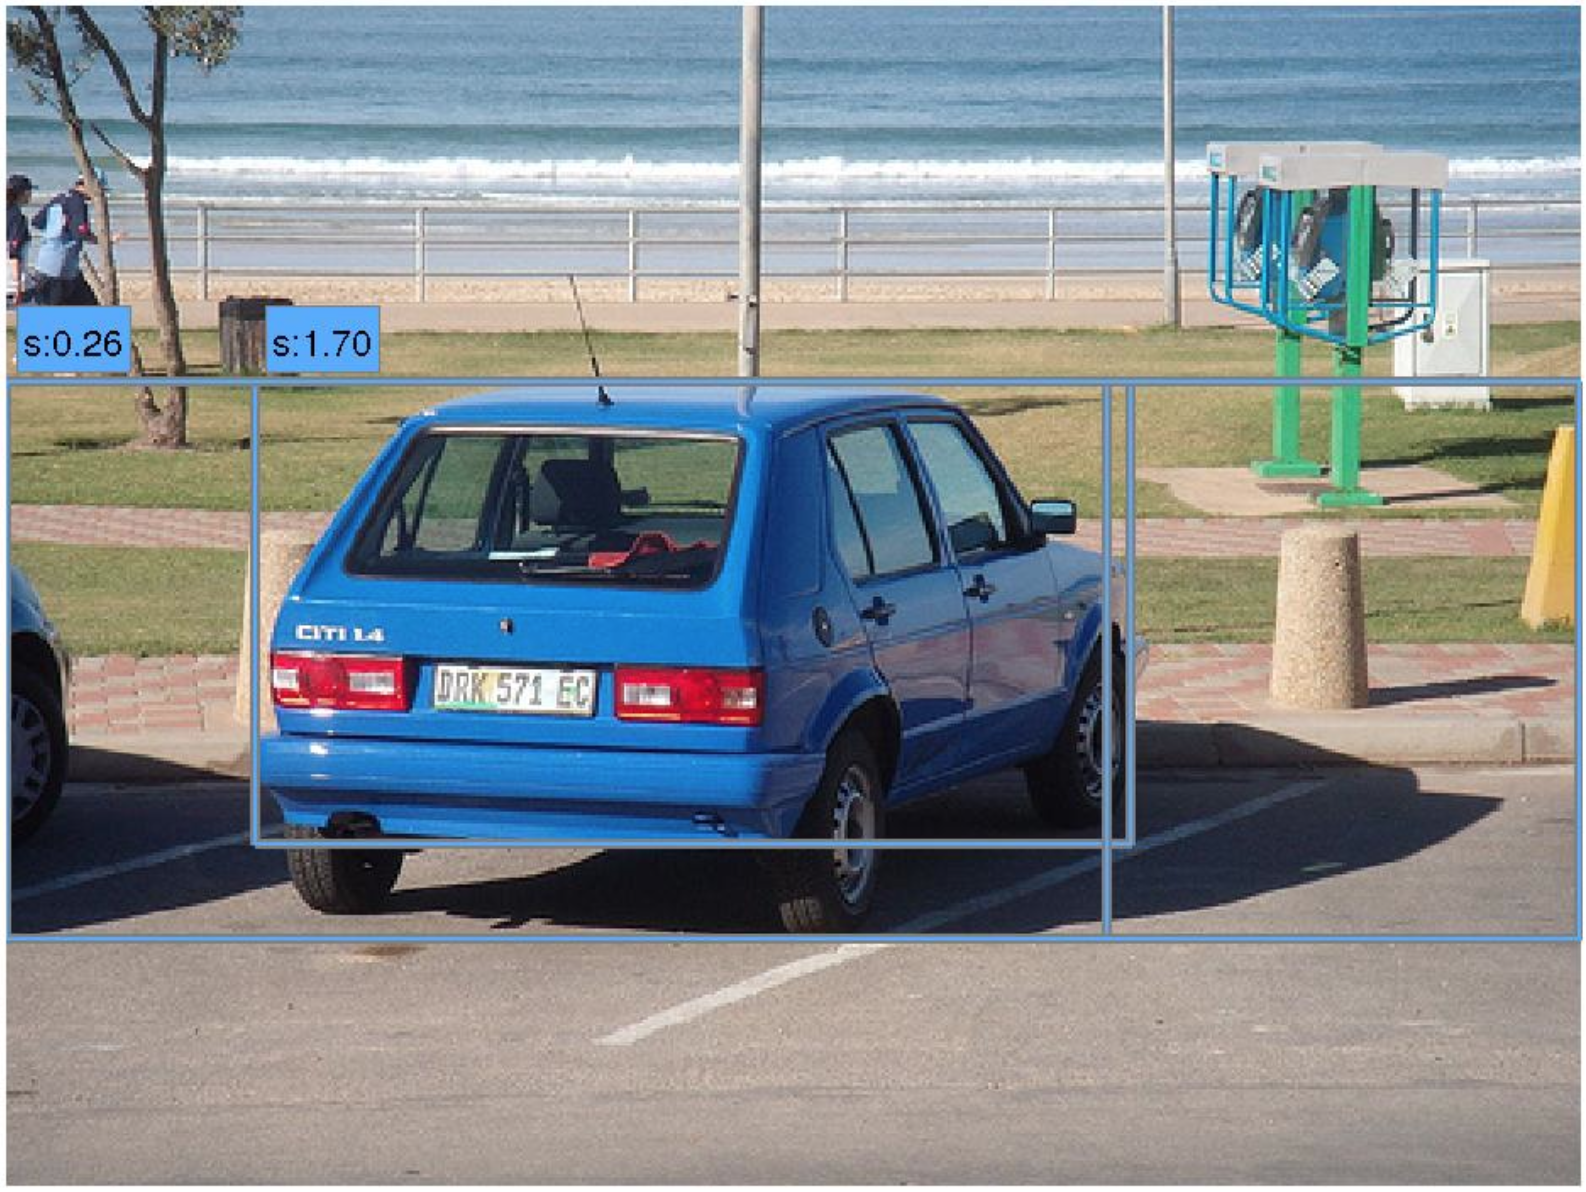
\includegraphics[width=0.24\textwidth]{bicycle_cnn/3a.png} &   
%   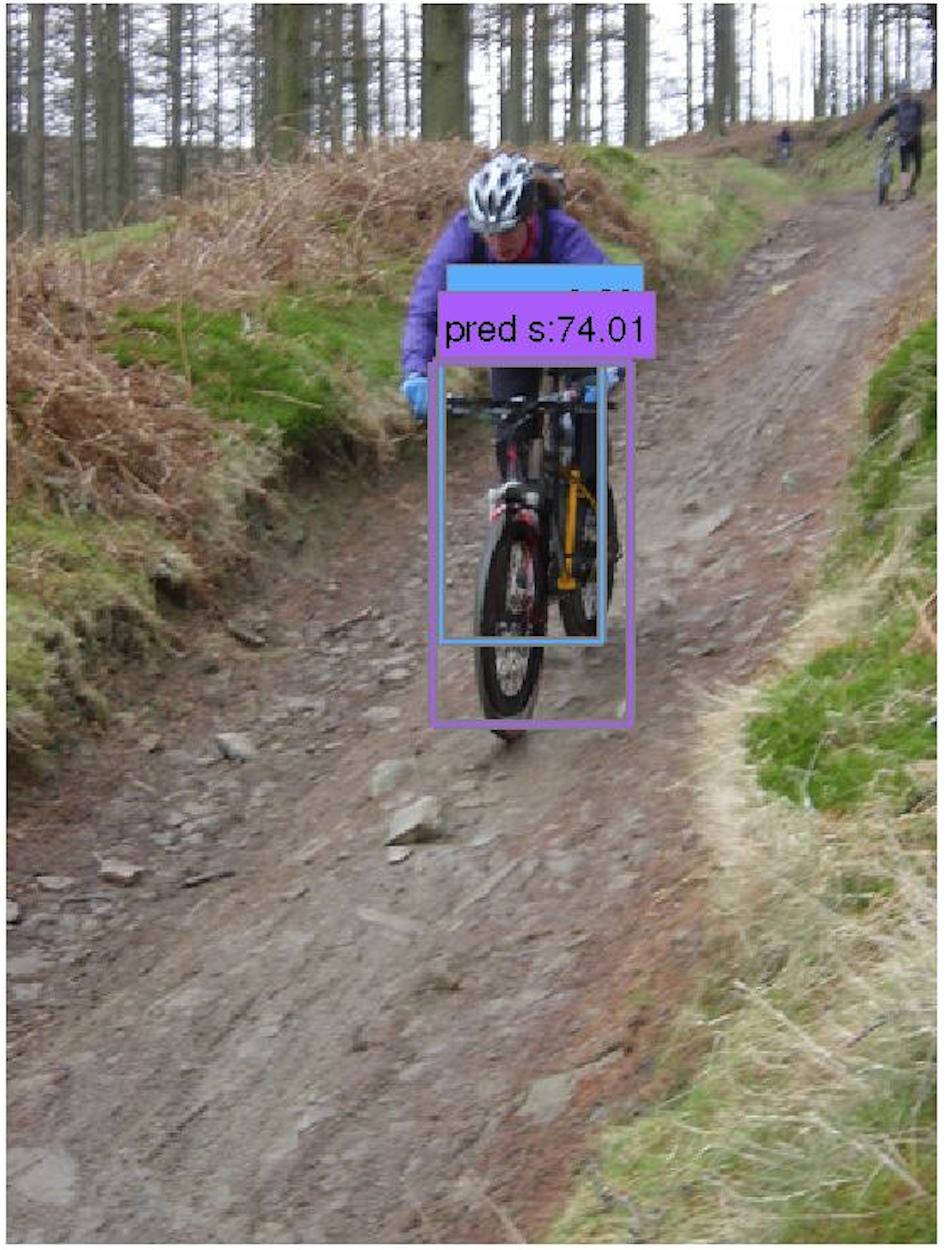
\includegraphics[width=0.24\textwidth]{bicycle_cnn/3b.png} &   
%   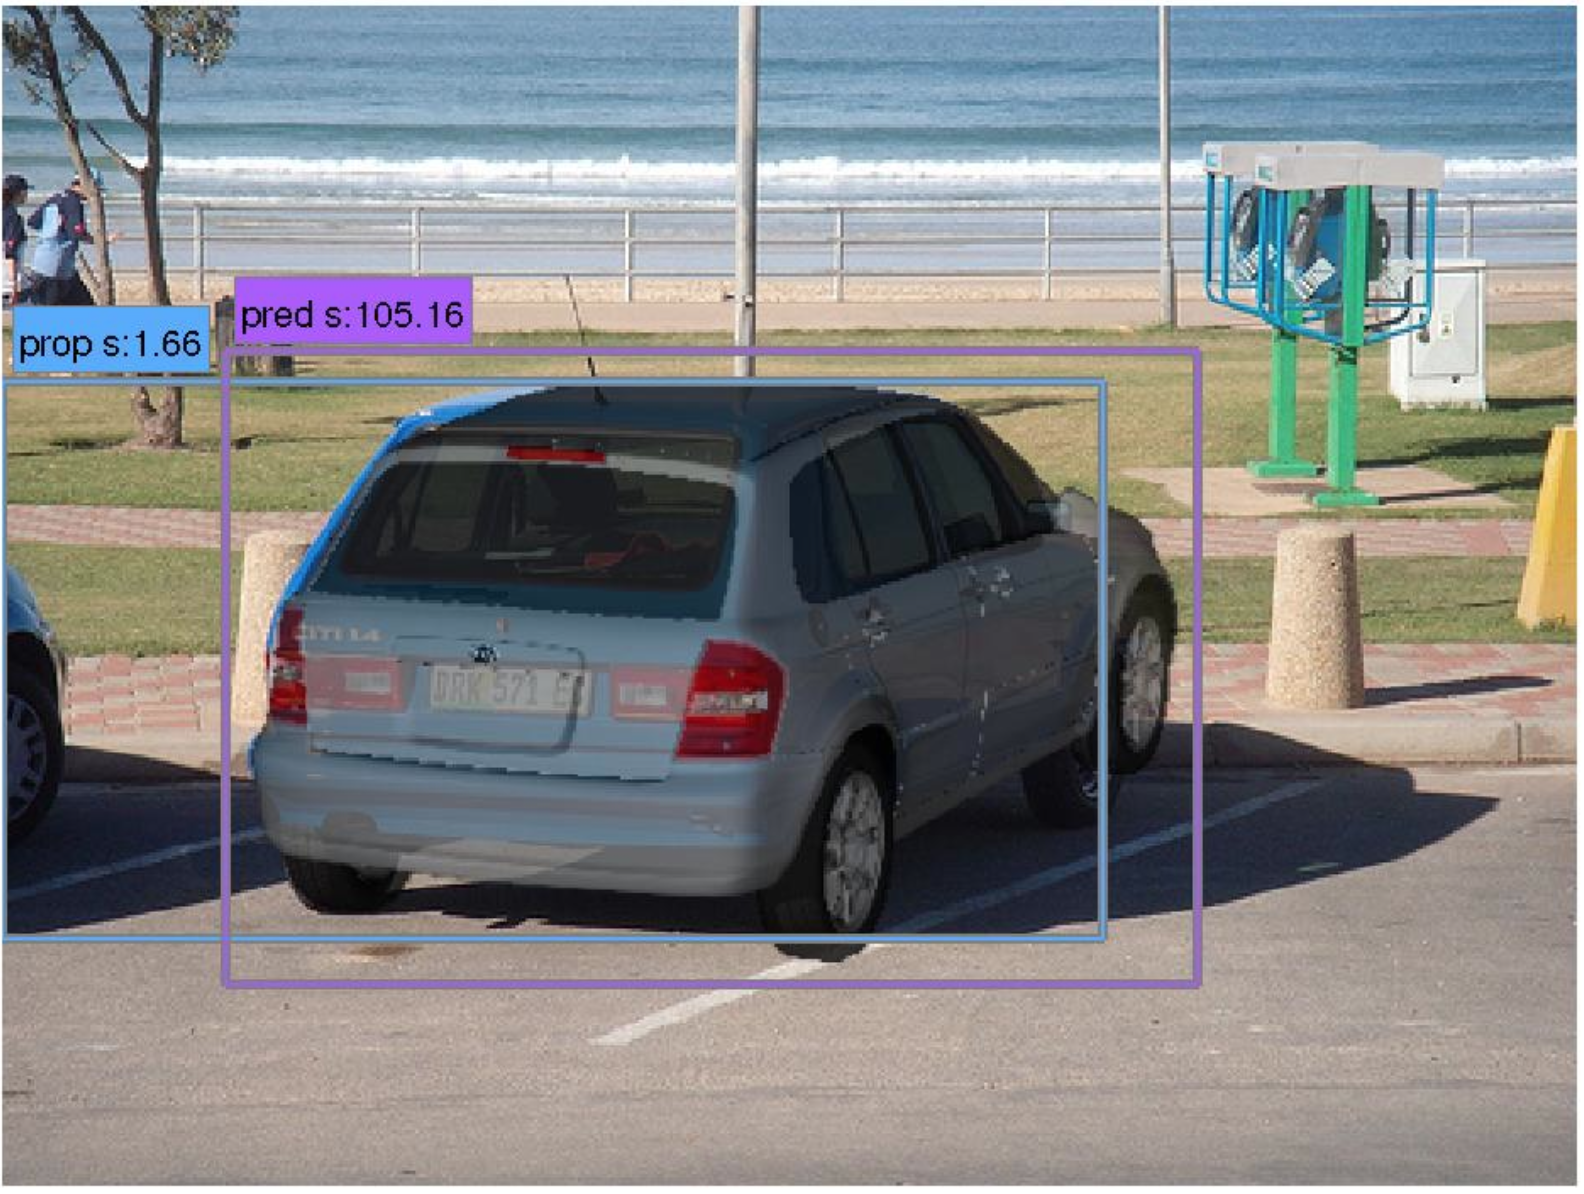
\includegraphics[width=0.24\textwidth]{bicycle_cnn/3c.png} &   
%   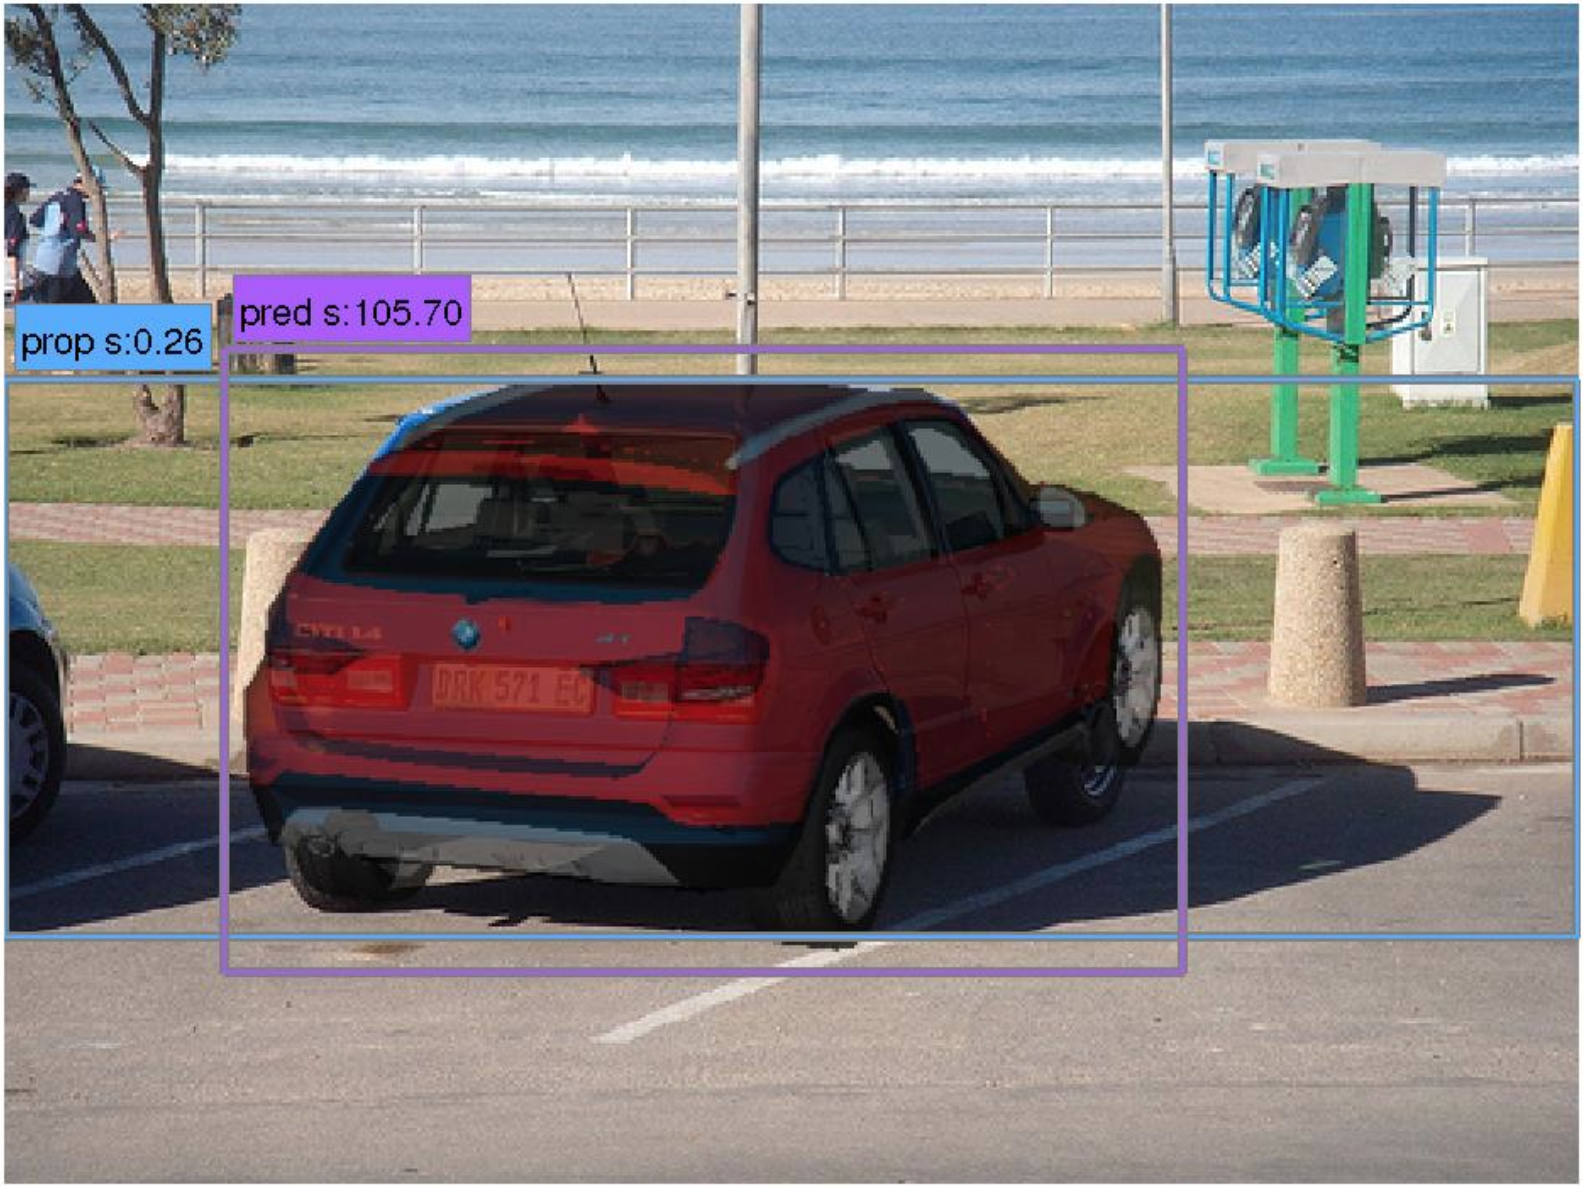
\includegraphics[width=0.24\textwidth]{bicycle_cnn/3d.png}  \\
  \hline
  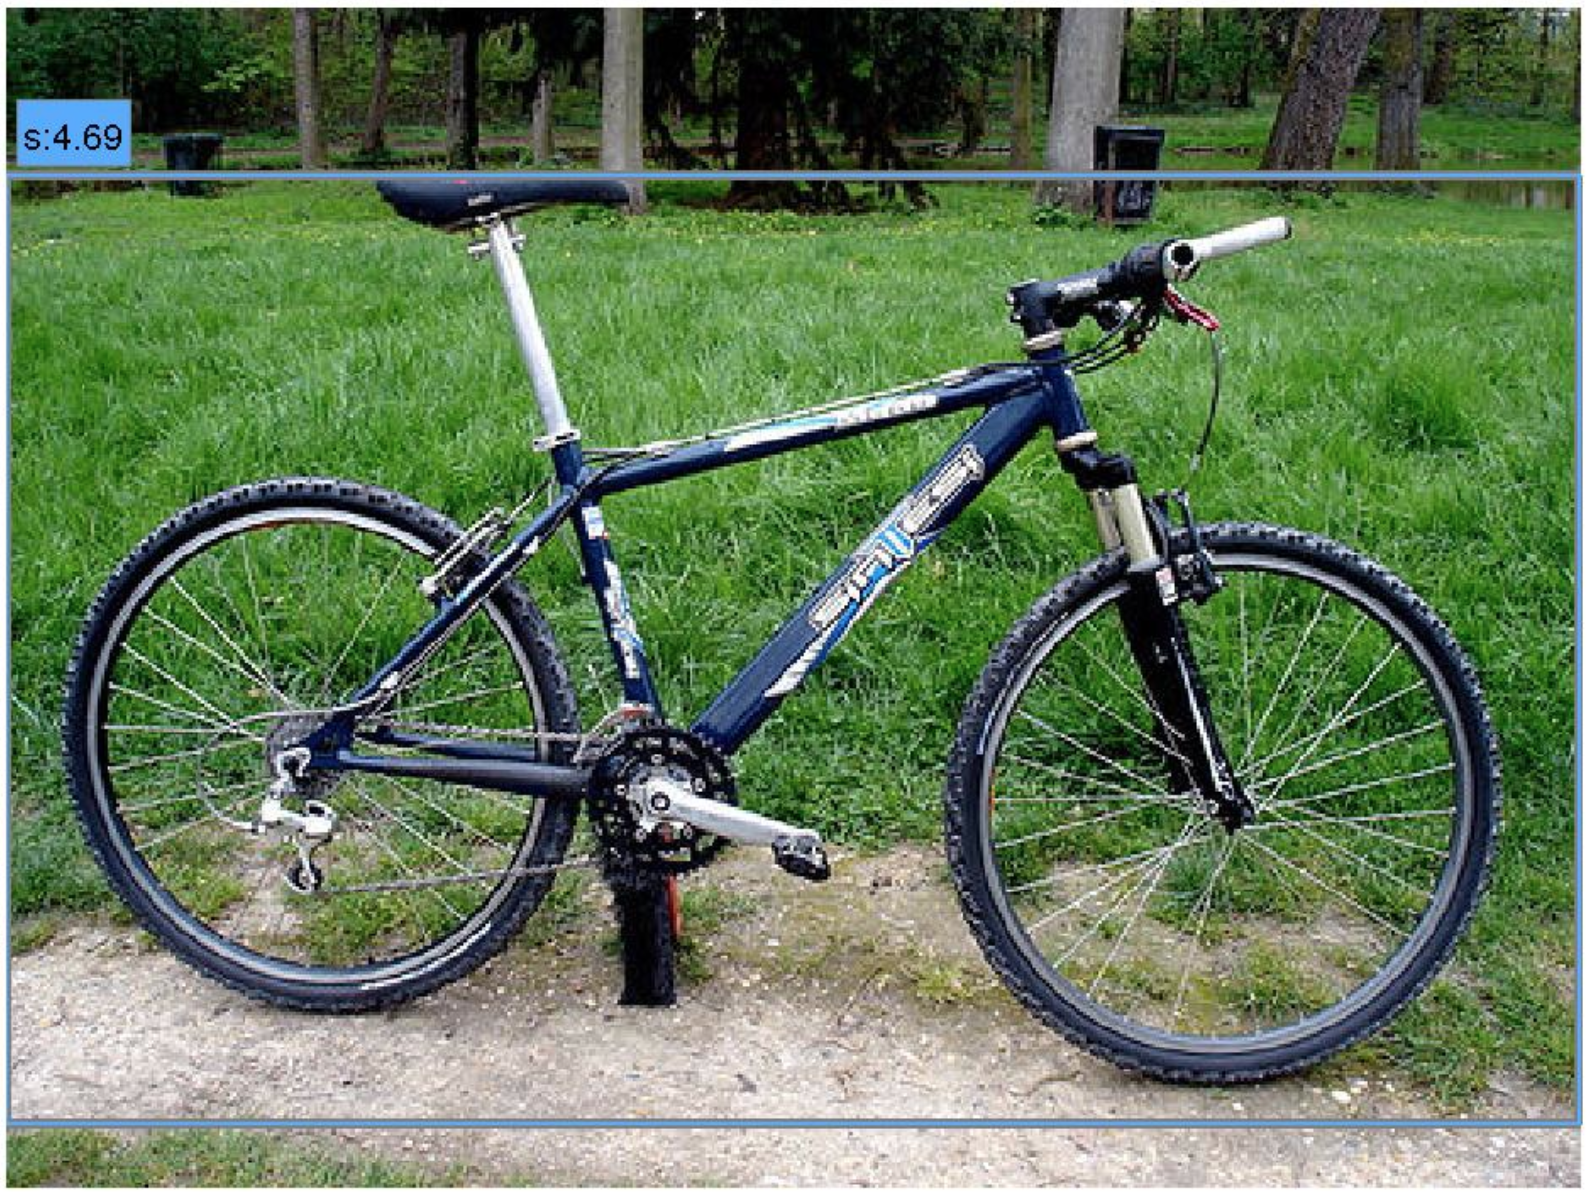
\includegraphics[width=0.24\textwidth]{bicycle_cnn/7a.png} &   
  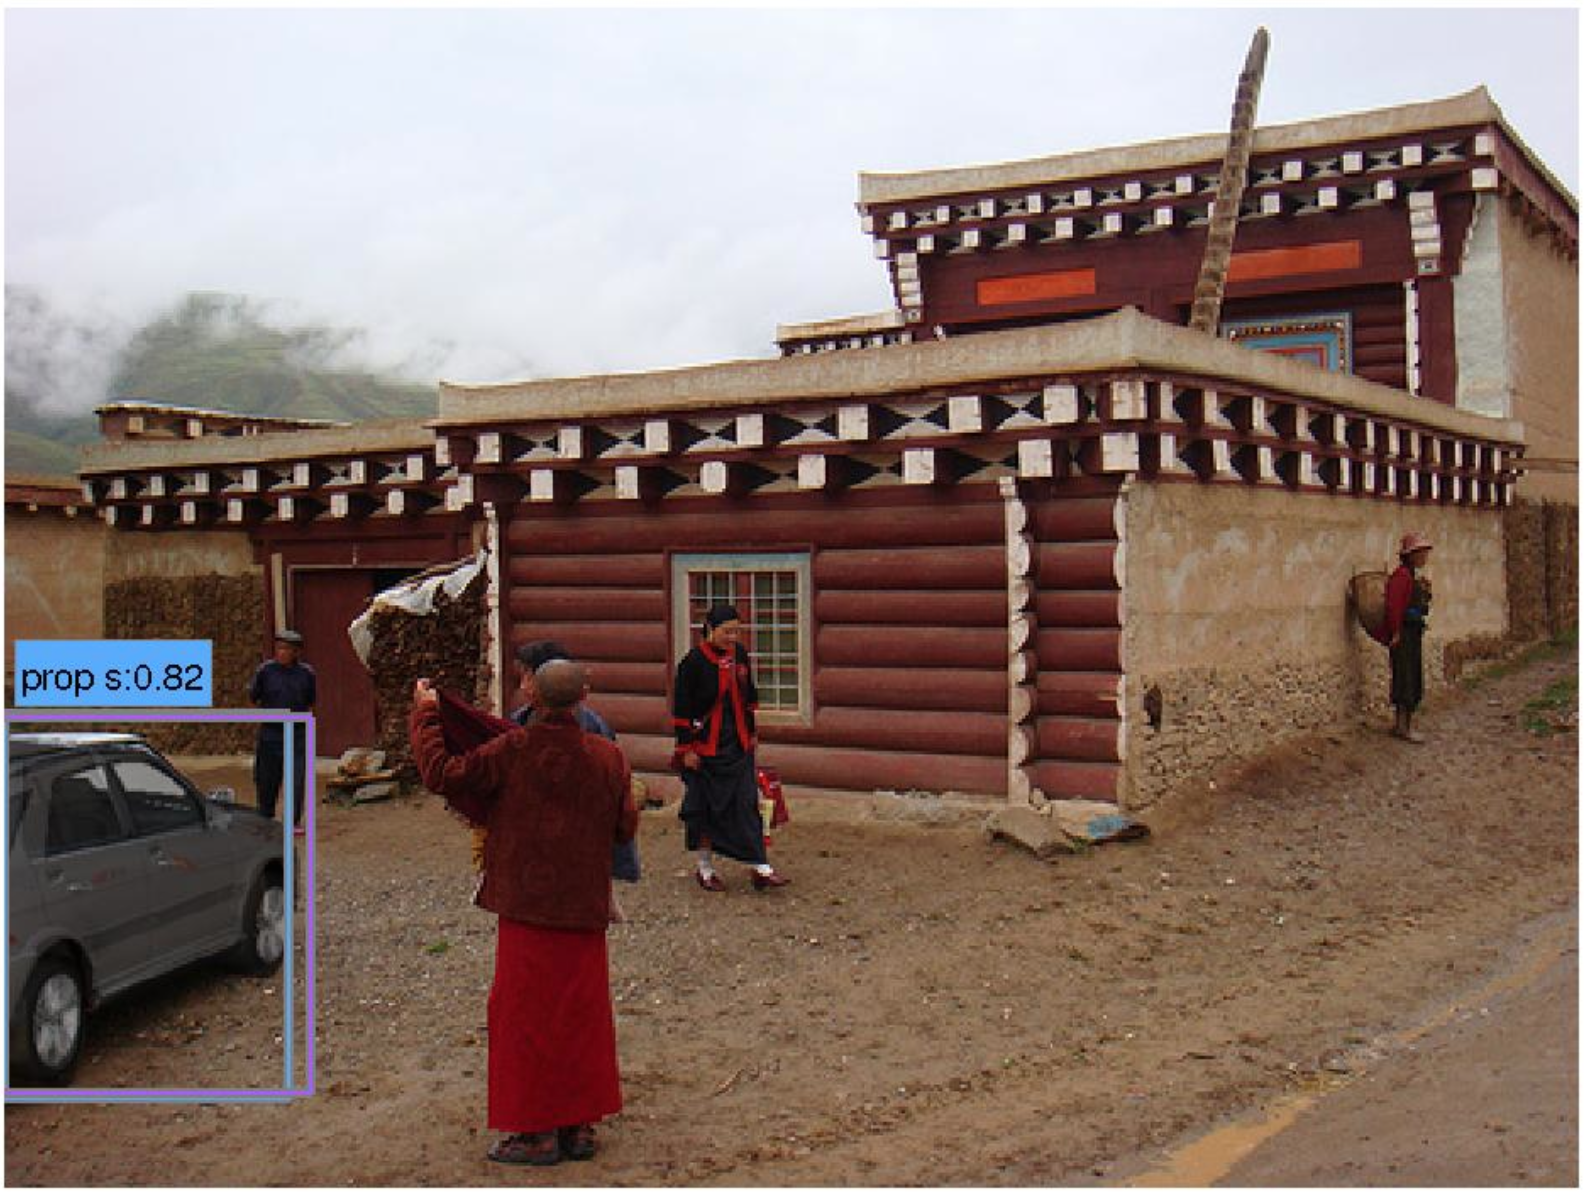
\includegraphics[width=0.24\textwidth]{bicycle_cnn/7b.png} &   
  &\\
  \hline
  \includegraphics[width=0.24\textwidth]{bicycle_cnn/4a.png} &   
  \includegraphics[width=0.24\textwidth]{bicycle_cnn/4b.png} &   
  \includegraphics[width=0.24\textwidth]{bicycle_cnn/4c.png} &   
  \includegraphics[width=0.24\textwidth]{bicycle_cnn/4d.png}  \\
  \hline
  CNN Proposals & \multicolumn{3}{|c|}{Our matching results on proposal bounding boxes} \\
  \hline
\end{tabular}
\caption{Example enriched bounding boxes. Given R-CNN\cite{Girshick14} detection bounding boxes, our method predicted 2D-3D matching reasonably. On the first column, R-CNN detection bounding boxes overlaid. From the second to the last columns, output of our method given a R-CNN box. Blue boxes are R-CNN output and purple boxes are the tightest bounding box enclosing predicted CAD model}
  \label{fig:pascal12cnn}
\end{figure*}
\begin{table*}[!htbp]
    \footnotesize
  \begin{center}
\begin{tabular}{|c|c|c|c|c|c|c|}
\hline
AP/AVP              & V-DPM \cite{Xiang14} & VOC-DPM \cite{Pepik12}  & \cite{Pepik12} + Ours (discrete) & \cite{Pepik12} + Ours (full) & R-CNN + Ours (discrete) & R-CNN + Ours (full)\\
\hline\hline
car-4v              & 37.2 / 20.2         & 45.6 / 36.9             & 47.6 / 42.7       & 47.6 / \textbf{42.7}        & 49.6 / 41.5         & 49.6 / 41.5\\ \hline
car-8v              & 37.3 / 23.5         & 47.6 / 36.6             & 47.6 / \textbf{39.8}       & 47.6 / 39.5        & 49.6 / 38.0         & 49.6 / 39.0\\ \hline
car-16v             & 36.6 / 18.1         & 46.0 / 29.6             & 47.6 / 32.7       & 47.6 / 33.0        & 49.6 / 34.0         & 49.6 / \textbf{34.3}\\ \hline
car-24v             & 36.3 / 13.7         & 42.1 / 24.6             & 47.6 / 27.4       & 47.6 / 27.4        & 49.6 / 27.0         & 49.6 / \textbf{27.6}\\ \hline
\hline
bicycle-4v          & 45.2 / 41.7         & 46.9 / 43.9             & 48.1 / 47.6       & 48.1 / 46.6        & 61.7 / 56.5         & 61.7 / \textbf{56.7}\\ \hline
bicycle-8v          & 47.3 / 36.7         & 48.1 / 40.3             & 48.1 / 40.6       & 48.1 / 40.6        & 61.7 / 48.9         & 61.7 / \textbf{49.2}\\ \hline
bicycle-16v         & 46.5 / 18.4         & 45.6 / 22.9             & 48.1 / 26.2       & 40.1 / 27.3        & 61.7 / 34.7         & 61.7 / \textbf{35.8}\\ \hline
bicycle-24v         & 44.4 / 14.3         & 45.9 / 16.7             & 48.1 / 21.5       & 40.1 / 20.9        & 61.7 / \textbf{27.0}         & 61.7 / 23.9\\ \hline
\end{tabular}
\end{center}
\caption{Average Precision(AP) and Average Viewpoint Precision(AVP) on PASCAL 3D dataset\cite{Xiang14}. For combined method (* + Ours), we use bounding boxes from * and augment viewpoint using our method. R-CNN and run our method to produce 2D-3D matching. If our method fails to give viewpoint, it predicts the viewpoint to be 0. Note that our method gives high quality metadata such as continuous 3D viewpoint, CAD model (rendering depth) and fine-grained category, whereas base-line methods gives 1D discrete azimuths. Our R-CNN was not an optimized version so the detection AP is lower than the state-of-the-art R-CNN performance}
\label{tab:pascal12}
\end{table*}

\begin{figure}[h]
\setlength\tabcolsep{1pt}
\centering
\begin{tabular}{cc}
  \hline
  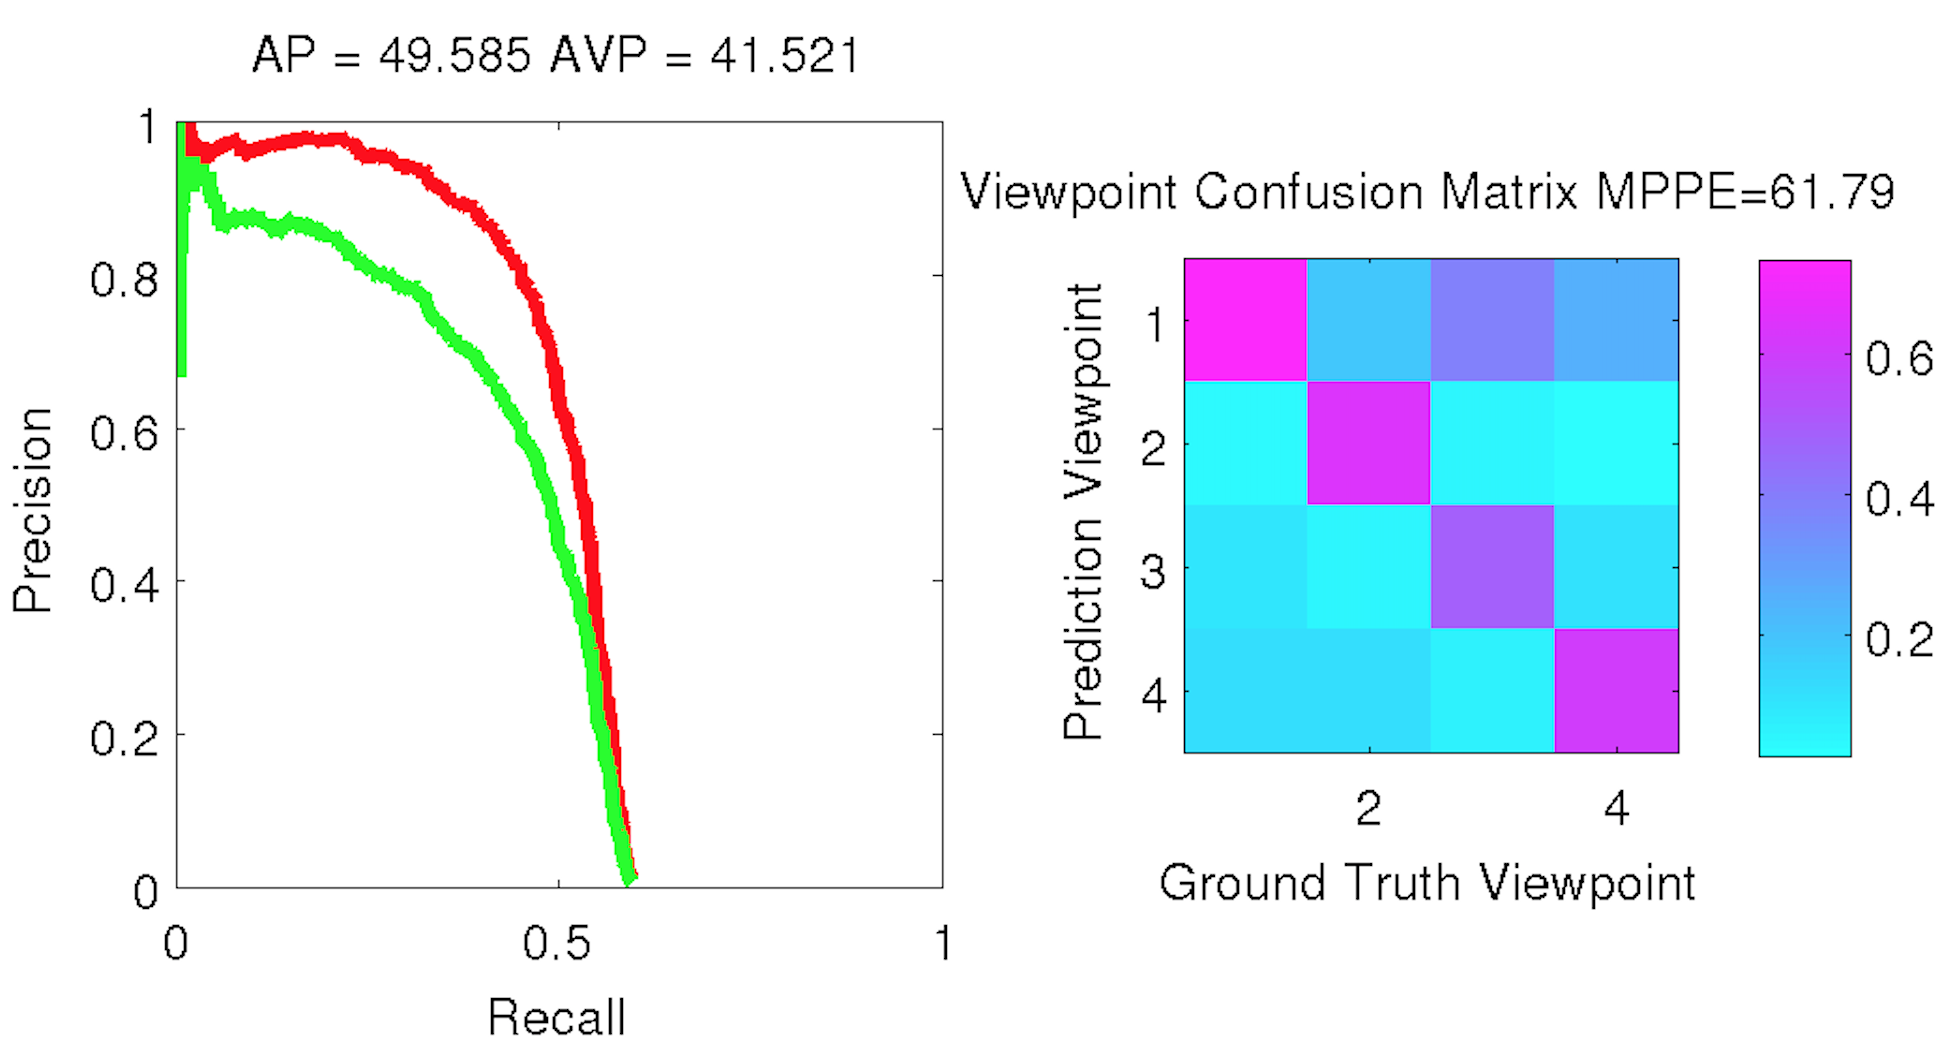
\includegraphics[width=0.49\linewidth]{car_cnn4_crop.png} &   
  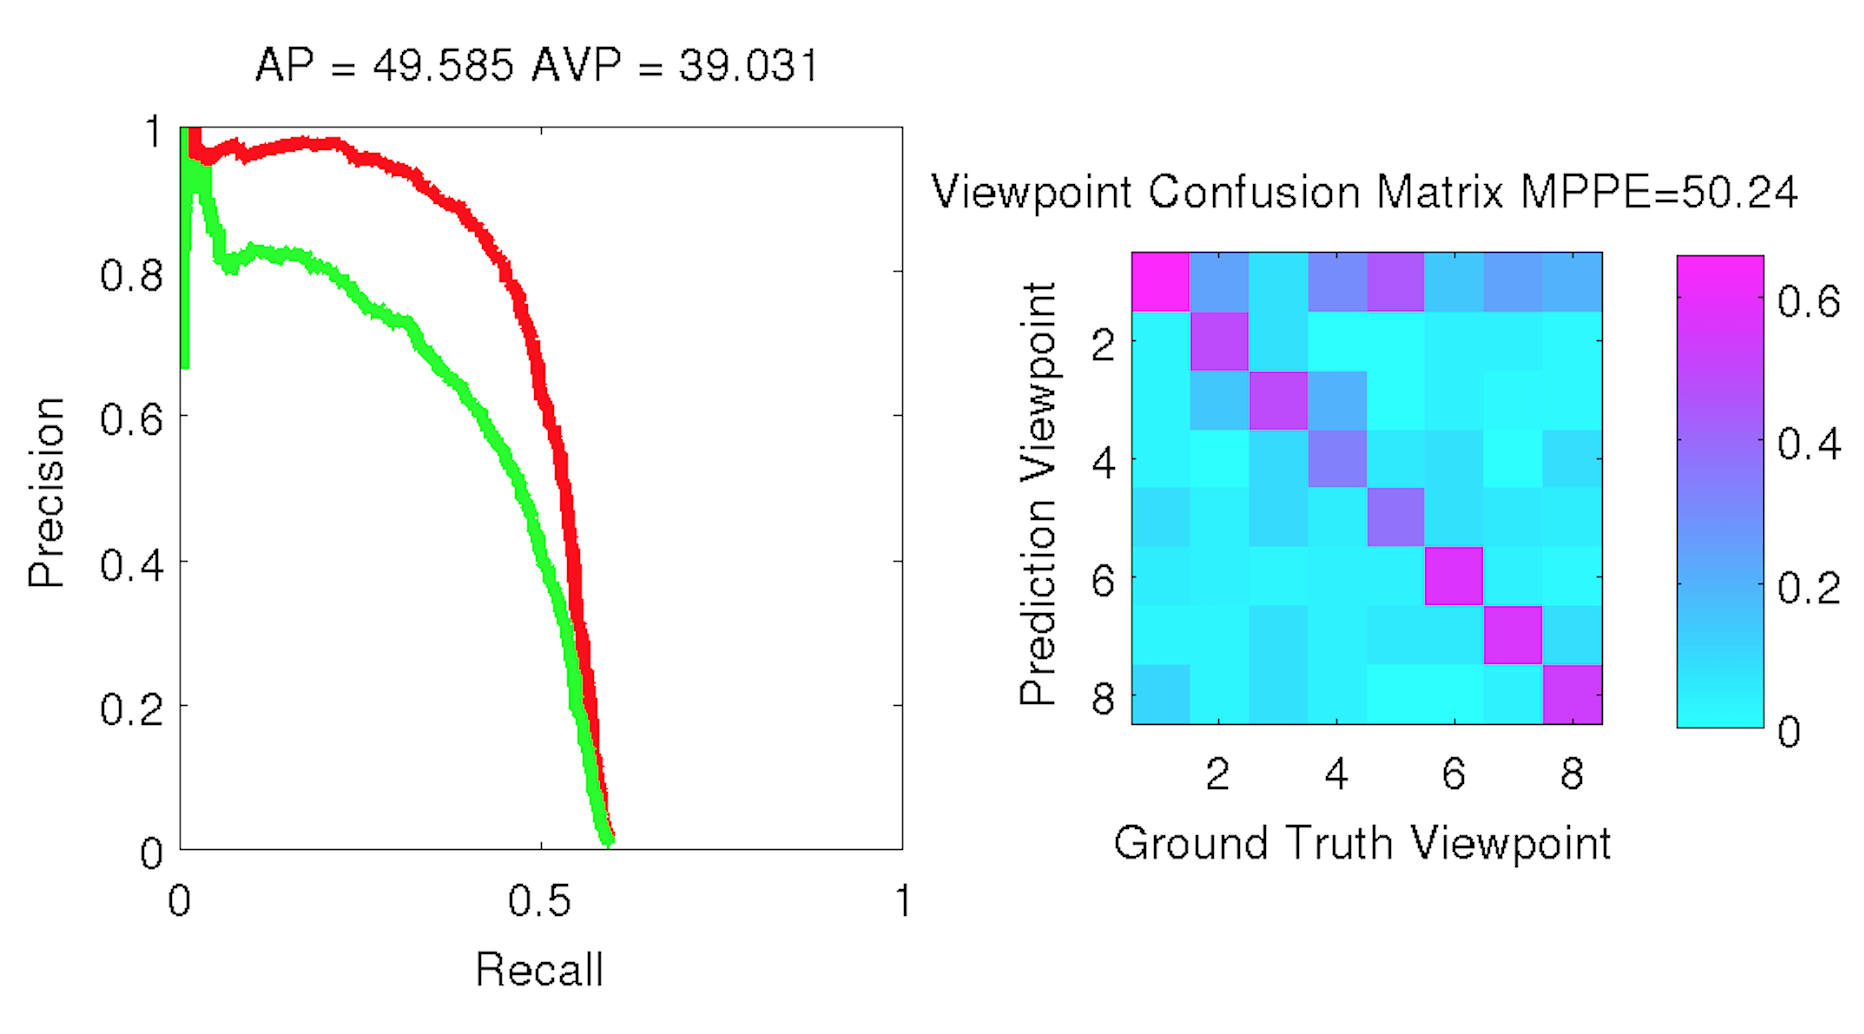
\includegraphics[width=0.49\linewidth]{car_cnn8_crop.png} \\   
  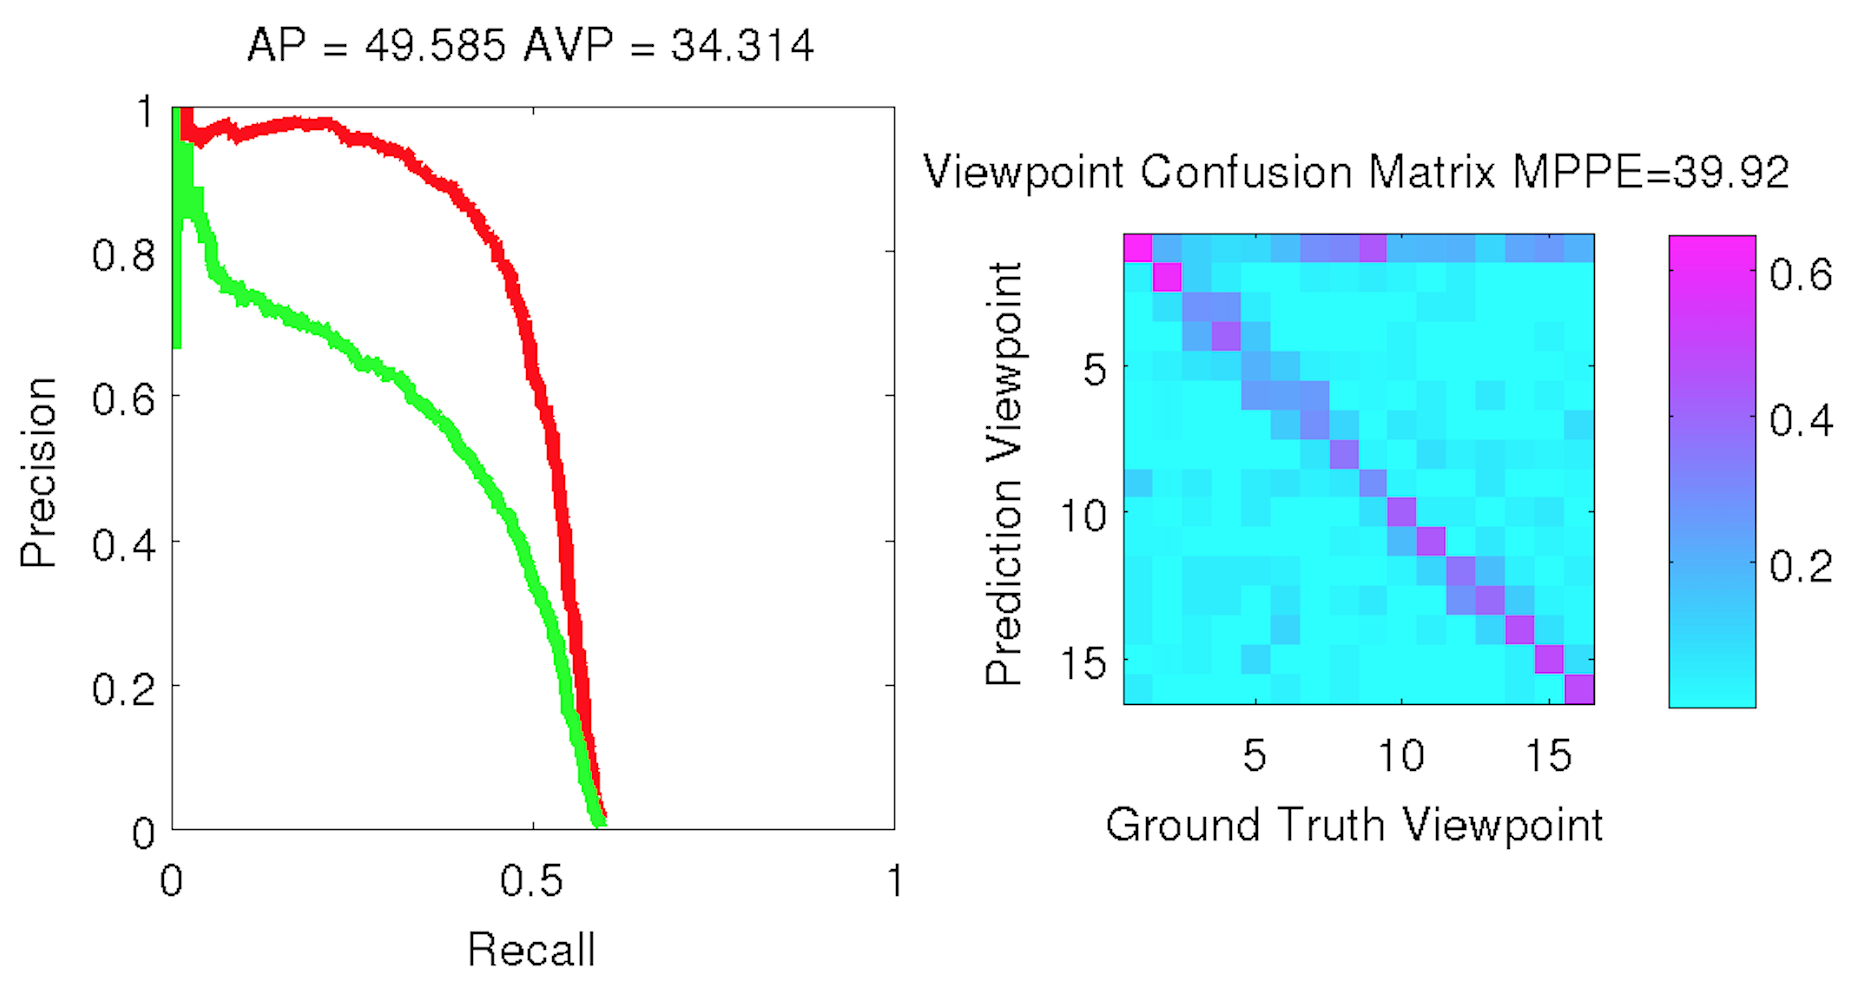
\includegraphics[width=0.49\linewidth]{car_cnn16_crop.png} &   
  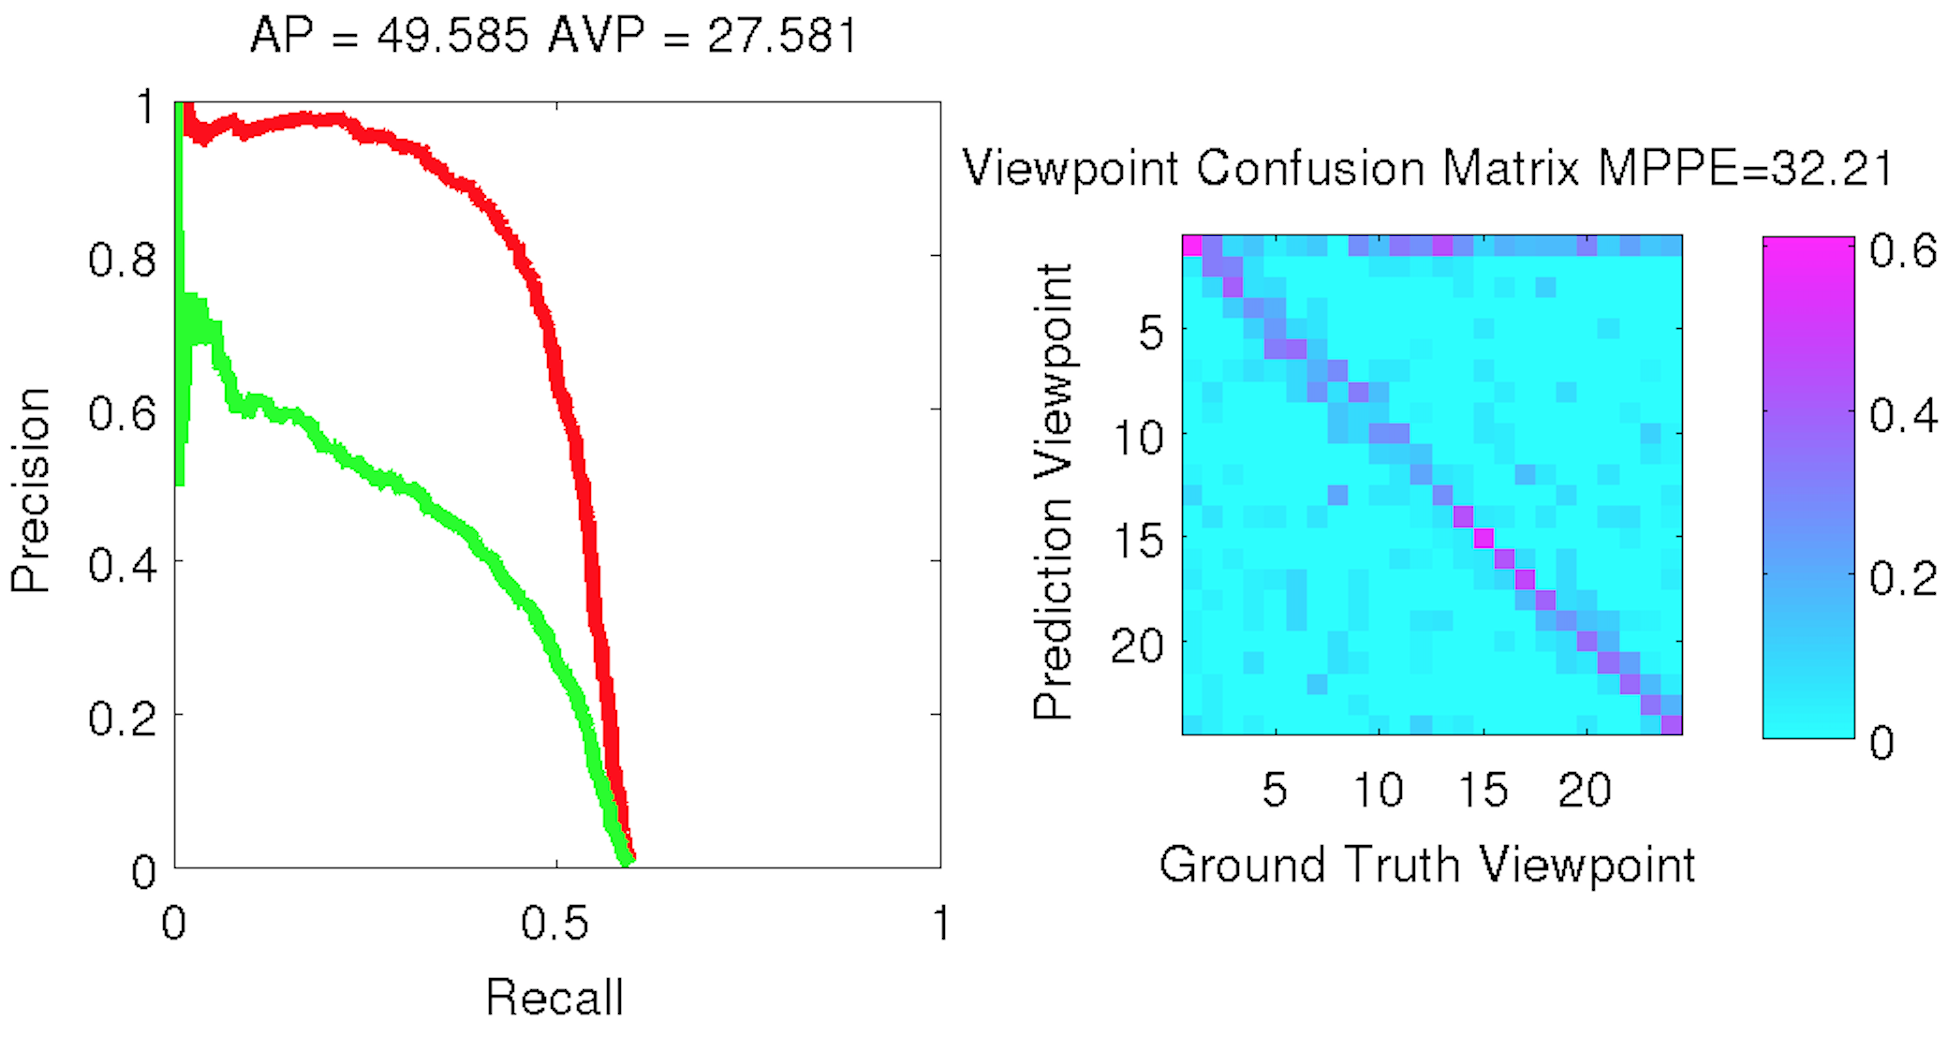
\includegraphics[width=0.49\linewidth]{car_cnn24_crop.png} \\   
  \hline
\end{tabular}
\caption{Average Precision (AP) and Average Viewpoint Precision (AVP) and viewpoint confusion table on PASCAL 12 car validation set using R-CNN + Ours. From the top left, 4 views, 8 views, 16 views and 24 views. Since our method only augment the object detection, the AP remains the same for all cases. As we increase the viewpoint estimation, the AVP decreases. Note that since we estimate null viewpoint if our method fails to find match, there are more 0 viewpoint predictions (top row of confusion matrices) }
  \label{fig:car_cnn_ap}
\end{figure}

\subsection{Stability of Our Method for Irregular Bounding Boxes}

% Generic object detectors give overlapping detection bounding boxes of the same object which can be handled by non maximal suppression. For these overlapping detections, 

R-CNN detection bounding boxes are irregular in shape since they come from other region proposal methods and sometimes they truncate objects. To handle such irregular shape and truncation, we added small context around the bounding boxes and run our method. 

We assumed that object can be arbitrarily truncated by the bounding box and search all plausible scales and translations. This can be efficiently computed using FFT-based convolution (refer Section. \ref{sec:fft}). We put examples of such conditions in Figure \ref{fig:stability}. Although the input bounding boxes are irregular and truncate objects, our method reliably generated a reasonable prediction of pose, translation, scale and CAD model.



\begin{figure}[h]
\setlength\tabcolsep{5pt}
\begin{tabular}{cc}
  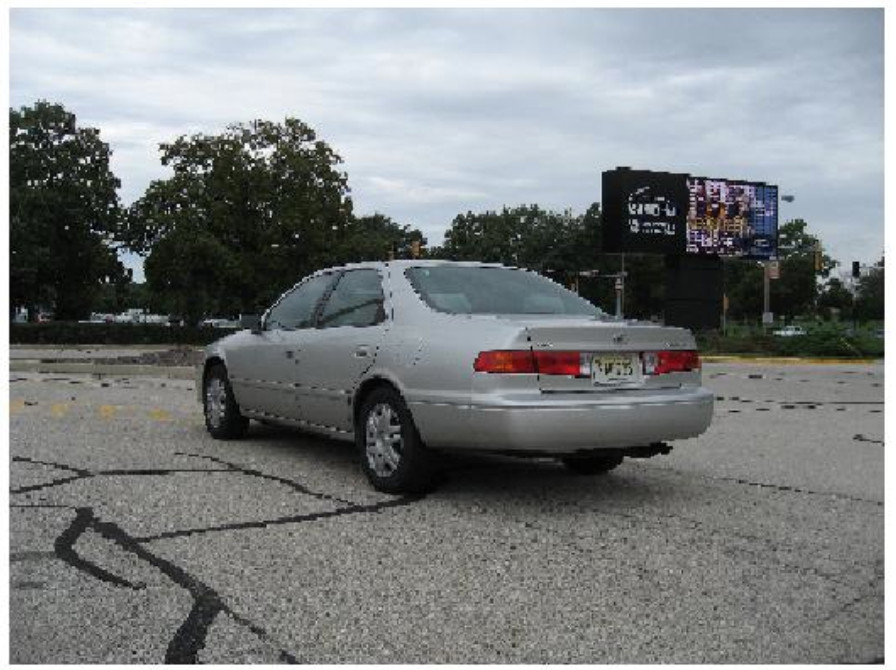
\includegraphics[width=0.45\linewidth]{car_pascal/1.png} &   
  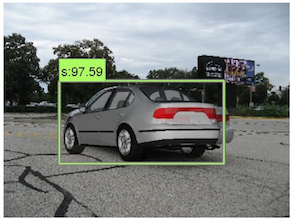
\includegraphics[width=0.45\linewidth]{car_pascal/2.png} \\   
  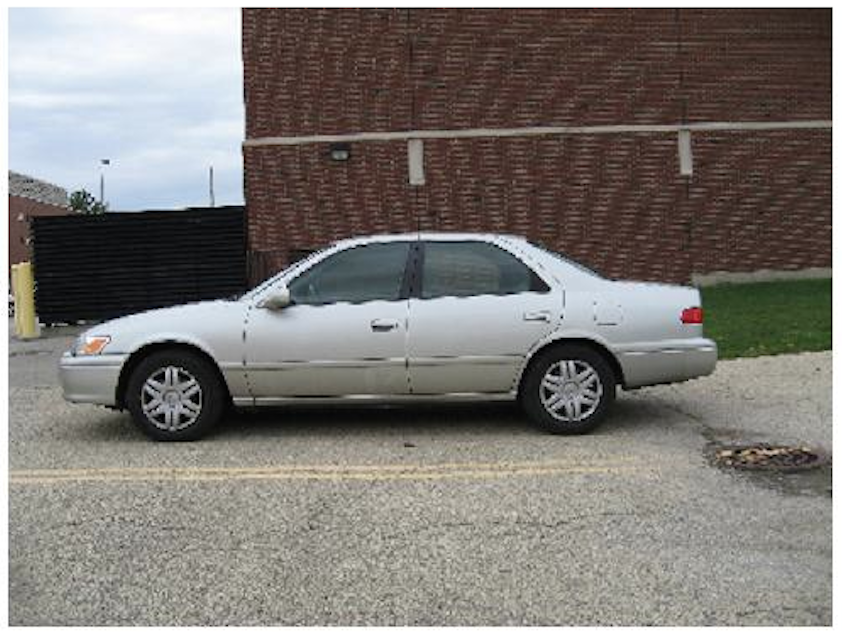
\includegraphics[width=0.45\linewidth]{car_pascal/3.png} &   
  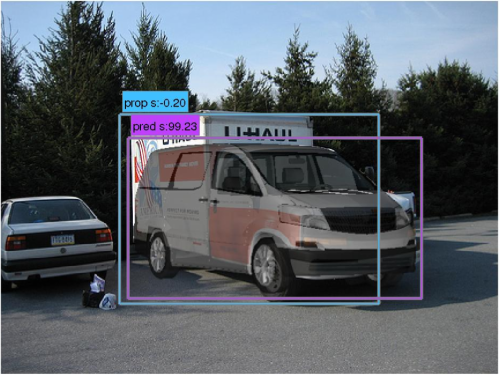
\includegraphics[width=0.45\linewidth]{car_pascal/4.png} \\   
\end{tabular}
\caption{Stability of our method for overlapping R-CNN detection \cite{Girshick14}. Blue box is the R-CNN detection that is feed into the system as initial detection. Purple box and overlaid rendering is the final output of the system. Note that for various overlapping bounding boxes, our system accurately estimated the reasonable result}
  \label{fig:stability}
\end{figure}


% For qualitative examples, we put hand-picked results from our method Fig. \ref{fig:car} and Fig. \ref{fig:bicycle}.

% \begin{figure*}[h]
% \setlength\tabcolsep{5pt}
% \begin{tabular}{|c|c|c|}
%     \hline
%   \includegraphics[width=0.325\textwidth]{car/PASCAL_car_val_init_0_Car_each_27_lim_250_lam_0_150_a_24_e_3_y_1_f_1_scale_2_00_sbin_6_level_15_skp_n_server_101_img_39.jpg} &   
%   \includegraphics[width=0.325\textwidth]{car/PASCAL_car_val_init_0_Car_each_27_lim_250_lam_0_150_a_24_e_3_y_1_f_1_scale_2_00_sbin_6_level_15_skp_n_server_101_img_78.jpg} & 
%   \includegraphics[width=0.325\textwidth]{car/PASCAL_car_val_init_0_Car_each_27_lim_250_lam_0_150_a_24_e_3_y_1_f_1_scale_2_00_sbin_6_level_15_skp_n_server_101_img_85.jpg} \\[-15pt]
% (a) & (b) & (c) \\[0pt]
% \hline
%   \includegraphics[width=0.325\textwidth]{car/PASCAL_car_val_init_0_Car_each_27_lim_250_lam_0_150_a_24_e_3_y_1_f_1_scale_2_00_sbin_6_level_15_skp_n_server_101_img_338.jpg} &   
%   \includegraphics[width=0.325\textwidth]{car/PASCAL_car_val_init_0_Car_each_27_lim_250_lam_0_150_a_24_e_3_y_1_f_1_scale_2_00_sbin_6_level_15_skp_n_server_101_img_360.jpg} & 
%   \includegraphics[width=0.325\textwidth]{car/PASCAL_car_val_init_0_Car_each_27_lim_250_lam_0_150_a_24_e_3_y_1_f_1_scale_2_00_sbin_6_level_15_skp_n_server_101_img_414.jpg} \\[-15pt]
% (d) & (e) & (f) \\[0pt]
% \hline
%   \includegraphics[width=0.325\textwidth]{car/PASCAL_car_val_init_0_Car_each_27_lim_250_lam_0_150_a_24_e_3_y_1_f_1_scale_2_00_sbin_6_level_15_skp_n_server_101_img_418.jpg} &   
%   \includegraphics[width=0.325\textwidth]{car/PASCAL_car_val_init_0_Car_each_27_lim_250_lam_0_150_a_24_e_3_y_1_f_1_scale_2_00_sbin_6_level_15_skp_n_server_101_img_1049.jpg} & 
%   \includegraphics[width=0.325\textwidth]{car/PASCAL_car_val_init_0_Car_each_27_lim_250_lam_0_150_a_24_e_3_y_1_f_1_scale_2_00_sbin_6_level_15_skp_n_server_101_img_1242.jpg} \\[-15pt]
% (g) & (h) & (i) \\[0pt]
% \hline
%   \includegraphics[width=0.325\textwidth]{car/PASCAL_car_val_init_0_Car_each_27_lim_250_lam_0_150_a_24_e_3_y_1_f_1_scale_2_00_sbin_6_level_15_skp_n_server_101_img_1244.jpg} &   
%   \includegraphics[width=0.325\textwidth]{car/PASCAL_car_val_init_0_Car_each_27_lim_250_lam_0_150_a_24_e_3_y_1_f_1_scale_2_00_sbin_6_level_15_skp_n_server_101_img_1261.jpg} & 
%   \includegraphics[width=0.325\textwidth]{car/PASCAL_car_val_init_0_Car_each_27_lim_250_lam_0_150_a_24_e_3_y_1_f_1_scale_2_00_sbin_6_level_15_skp_n_server_101_img_1452.jpg} \\[-15pt]
% (j) & (k) & (l) \\[0pt]
% \hline
%   \includegraphics[width=0.325\textwidth]{car/PASCAL_car_val_init_0_Car_each_27_lim_250_lam_0_150_a_24_e_3_y_1_f_1_scale_2_00_sbin_6_level_15_skp_n_server_101_img_1467.jpg} &   
%   \includegraphics[width=0.325\textwidth]{car/PASCAL_car_val_init_0_Car_each_27_lim_250_lam_0_150_a_24_e_3_y_1_f_1_scale_2_00_sbin_6_level_15_skp_n_server_101_img_1553.jpg} & 
%   \includegraphics[width=0.325\textwidth]{car/PASCAL_car_val_init_0_Car_each_27_lim_250_lam_0_150_a_24_e_3_y_1_f_1_scale_2_00_sbin_6_level_15_skp_n_server_101_img_1597.jpg} \\[-15pt]
% (m) & (n) & (o) \\[3pt]
% \hline
% \end{tabular}
%   \caption{Selected detections from PASCAL 07 Car categories. From the left, (1) original image, (2) overlaid true positive CAD models, (3) overlaid true positive CAD models with bounding boxes, (4) overlaid false positive CAD models with bounding boxes. Bounding box is colored from red (high confidence) to blue (low confidence) }
%   \label{fig:car}
% \end{figure*}
% \begin{figure*}[h]
% \setlength\tabcolsep{5pt}
% \begin{tabular}{|c|c|c|}
%     \hline
%   \includegraphics[width=0.325\textwidth]{bicycle/PASCAL_bicycle_val_init_0_Bicycle_each_4_lim_250_lam_0_150_a_48_e_4_y_5_f_1_scale_2_00_sbin_6_level_15_skp_n_server_102_img_459.jpg} &   
%   \includegraphics[width=0.325\textwidth]{bicycle/PASCAL_bicycle_val_init_0_Bicycle_each_4_lim_250_lam_0_150_a_48_e_4_y_5_f_1_scale_2_00_sbin_6_level_15_skp_n_server_102_img_1300.jpg} &   
%   \includegraphics[width=0.325\textwidth]{bicycle/PASCAL_bicycle_val_init_0_Bicycle_each_4_lim_250_lam_0_150_a_48_e_4_y_5_f_1_scale_2_00_sbin_6_level_15_skp_n_server_102_img_539.jpg} \\[-15pt]
% (a) & (b) & (c) \\[0pt]
% \hline
%   \includegraphics[width=0.325\textwidth]{bicycle/PASCAL_bicycle_val_init_0_Bicycle_each_4_lim_250_lam_0_150_a_48_e_4_y_5_f_1_scale_2_00_sbin_6_level_15_skp_n_server_102_img_35.jpg} &   
%   \includegraphics[width=0.325\textwidth]{bicycle/PASCAL_bicycle_val_init_0_Bicycle_each_4_lim_250_lam_0_150_a_48_e_4_y_5_f_1_scale_2_00_sbin_6_level_15_skp_n_server_102_img_83.jpg} &   
%   \includegraphics[width=0.325\textwidth]{bicycle/PASCAL_bicycle_val_init_0_Bicycle_each_4_lim_250_lam_0_150_a_48_e_4_y_5_f_1_scale_2_00_sbin_6_level_15_skp_n_server_102_img_131.jpg} \\[-15pt]
% (d) & (e) & (f) \\[0pt]
% \hline
%   \includegraphics[width=0.325\textwidth]{bicycle/PASCAL_bicycle_val_init_0_Bicycle_each_4_lim_250_lam_0_150_a_48_e_4_y_5_f_1_scale_2_00_sbin_6_level_15_skp_n_server_102_img_175.jpg} &   
%   \includegraphics[width=0.325\textwidth]{bicycle/PASCAL_bicycle_val_init_0_Bicycle_each_4_lim_250_lam_0_150_a_48_e_4_y_5_f_1_scale_2_00_sbin_6_level_15_skp_n_server_102_img_210.jpg} &   
%   \includegraphics[width=0.325\textwidth]{bicycle/PASCAL_bicycle_val_init_0_Bicycle_each_4_lim_250_lam_0_150_a_48_e_4_y_5_f_1_scale_2_00_sbin_6_level_15_skp_n_server_102_img_233.jpg} \\[-15pt]
% (g) & (h) & (i) \\[0pt]
% \hline
%   \includegraphics[width=0.325\textwidth]{bicycle/PASCAL_bicycle_val_init_0_Bicycle_each_4_lim_250_lam_0_150_a_48_e_4_y_5_f_1_scale_2_00_sbin_6_level_15_skp_n_server_102_img_322.jpg} &   
%   \includegraphics[width=0.325\textwidth]{bicycle/PASCAL_bicycle_val_init_0_Bicycle_each_4_lim_250_lam_0_150_a_48_e_4_y_5_f_1_scale_2_00_sbin_6_level_15_skp_n_server_102_img_348.jpg} &   
%   \includegraphics[width=0.325\textwidth]{bicycle/PASCAL_bicycle_val_init_0_Bicycle_each_4_lim_250_lam_0_150_a_48_e_4_y_5_f_1_scale_2_00_sbin_6_level_15_skp_n_server_102_img_375.jpg} \\[-15pt]
% (j) & (k) & (l) \\[0pt]
% \hline
%   \includegraphics[width=0.325\textwidth]{bicycle/PASCAL_bicycle_val_init_0_Bicycle_each_4_lim_250_lam_0_150_a_48_e_4_y_5_f_1_scale_2_00_sbin_6_level_15_skp_n_server_102_img_400.jpg} &   
%   \includegraphics[width=0.325\textwidth]{bicycle/PASCAL_bicycle_val_init_0_Bicycle_each_4_lim_250_lam_0_150_a_48_e_4_y_5_f_1_scale_2_00_sbin_6_level_15_skp_n_server_102_img_434.jpg} &   
%   \includegraphics[width=0.325\textwidth]{bicycle/PASCAL_bicycle_val_init_0_Bicycle_each_4_lim_250_lam_0_150_a_48_e_4_y_5_f_1_scale_2_00_sbin_6_level_15_skp_n_server_102_img_459.jpg} \\[-15pt]
% (m) & (n) & (o) \\[3pt]
% \hline
% \end{tabular}
%   \caption{Selected detections from PASCAL 12 Bike categories. From the left, (1) original image, (2) overlaid true positive CAD models, (3) overlaid true positive CAD models with bounding boxes, (4) overlaid false positive CAD models with bounding boxes. Bounding box is colored from red (high confidence) to blue (low confidence) }
%   \label{fig:bicycle}
% \end{figure*}


% \section{Object Detection with various Training Data}
% \section{Image Query}
